%! Composition : pdftex
\documentclass{scrreprt}
\usepackage[colorlinks=true]{hyperref}
\usepackage[utf8]{inputenc}
\usepackage[french]{babel}
\usepackage[T1]{fontenc}
\usepackage{graphicx}
\usepackage{fourier}
%\usepackage{lmodern}
\usepackage{helvet}
%\usepackage[scaled]{helvet}
\renewcommand{\familydefault}{\sfdefault}
\usepackage[a4paper, hmargin=113pt, vmargin=111pt]{geometry}
%\usepackage[bindingoffset=5mm]{geometry}
\usepackage{microtype}
\usepackage[hidelinks]{hyperref}
%\usepackage{microtype}%meilleur réglage espaces typo, pb avec les -- dans les tableaux
\usepackage{pdflscape}
\usepackage{longtablex}
\usepackage{tabularx}
\usepackage{multirow}
\usepackage{calc}
\usepackage{wrapfig}
\usepackage{xcolor}
\usepackage{pdfpages}
\usepackage{epigraph}
%\usepackage{scrtime}%heure système
\usepackage{fancyhdr}
\usepackage{titling}


%\usepackage{showframe}
\usepackage{layout}
%\usepackage{lipsum}

\graphicspath{{images/}}
\newlength{\HauteurTexte}
\setlength{\HauteurTexte}{\textheight}

\hypersetup{
    pdftitle={La germination},
    pdfauthor={Pachot, Alexandre},
    pdfsubject={Dossier CRPE 2015},
    pdfkeywords={Germination, PS, MS, maternelle, éducation}
}

\pagestyle{fancy}
%\lhead{}
%\chead{\thetitle}
%\rhead{} 
%\cfoot{\thepage}
\renewcommand{\headrulewidth}{0pt}

%\KOMAoptions{%
%	paper=a4,
%	fontsize=12pt,
%	DIV=calc,
%%	BCOR=5mm,
%%	twoside=on,
%}
\usepackage{helvet}
\renewcommand{\familydefault}{\sfdefault}

%Colophon
\newcommand{\police}{Helvetica}
\KOMAoptions{%
	paper=a4,
	fontsize=12pt,
	DIV=calc,
%	BCOR=5mm,
%	twoside=on,
}
\setboolean{caco}{false}
\setboolean{papier}{false}
\begin{document}
	%\layout{}
	\title{La germination en petite et moyenne section}
\author{Alexandre \textsc{Pachot}}
\date{}
\maketitle
	% Prologue
	\ifthenelse{\boolean{papier}}{\clearemptydoublepage}{}
\ifthenelse{\boolean{caco}}{}{\thispagestyle{empty}\pagenumbering{roman}}
~
\vfill

\hfill Tout savoir scientifique doit être à tout moment reconstruit.

\hfill \emph{La formation de l’esprit scientifique}

\hfill Gaston \textsc{Bachelard}
\vfill
\vfill
\vfill
	\ifthenelse{\boolean{caco}}{\newpage}{\clearemptydoublepage\thispagestyle{empty}}
\
\vfill
\begin{center}
	
\includegraphics[scale=.5]{orthographe}\\[1em]
	Ce document applique les rectifications orthographiques proposées par le Conseil supérieur de la langue française, approuvées par l’Académie française et publiées en décembre 1990 dans les \og Documents administratifs \fg{} du \emph{Journal officiel de la République française}.
\end{center}
	\ifthenelse{\boolean{papier}}{\clearemptydoublepage}{}
\ifthenelse{\boolean{caco}}{%
	\mbox{}\newpage
	\ifodd\thepage ~\newpage~\fi
	}{\chapter*{Résumé}}
Le programme d’enseignement de l’école primaire spécifie la démarche d’investigation pour l’enseignement des sciences au cycle~3, le site internet du Ministère de l’Éducation nationale, de l’Enseignement supérieur et de la Recherche préconise une initiation à la démarche d’investigation dès la maternelle, et le socle commun de connaissances et de compétences qui se retrouve dans le code de l’éducation fait référence à l’opération \og La main à la pâte \fg{} pour l’enseignement des sciences. D'après notre enquête, l’enseignement des sciences se fait effectivement dès la maternelle en utilisant cette démarche, et le nombre d’heures consacrées est proche du nombre d’heures consacré aux sciences au cycle~2. Néanmoins les dérives soulignées par le \textit{Rapport sur l’opération \og La main à la pâte \fg{} et l’enseignement des sciences à l’école primaire} sont toujours d’actualité. Il s’agit de la dérive du \og tout méthodologique \fg{} où l’utilisation de la démarche est privilégiée à l’acquisition des connaissances, ainsi que la dérive du \og tout technologique \fg{} où le seul but est de construire un objet sans que cela réponde à une problématique.

\begin{description}
\item[Mots-clés:] Éducation, sciences, maternelle, démarche d’investigation, La main à la pâte
\end{description}
\vfill
\ifthenelse{\boolean{papier}}{\clearemptydoublepage}{}
\ifthenelse{\boolean{caco}}{}{\chapter*{Abstract}}
\selectlanguage{english}
The curriculum of primary school specify the investigative approach for cycle~III (8–10 years of age), the website of the Ministry of National Education, Higher Education and Research recommends an introduction to the investigative approach in pre-school (3–5 years of age), and the Common Base of Knowledge and Skills that is found in the Education Code refers to the ``Hands on'' operation for teaching Science. According to our survey, science teaching in pre-school is actually using this approach, and the number of hours spent is close to the number of hours devoted to science in cycle II (6–7 years of age). Nevertheless drifts highlighted by the \textit{Report on the ``Hands on'' operation and science education in primary school} are still relevant. It is the drift of ``all methodological'' where the use of the approach is preferred to the acquisition of knowledge and the drift of ``all technological'' where the only goal is to construct an object that is not consistent with a problem.

\begin{description}
\item[Keywords:] Education, science, pre-school, investigation approach, Hands on
\end{description}
\selectlanguage{french}
\vfill
	\ifthenelse{\boolean{papier}}{\clearemptydoublepage}{}
\chapter*{Remerciements}
Je remercie :
\begin{itemize}
\item Bernard Chirol pour son accompagnement dans la réalisation de ce mémoire ;
\item les enseignantes de l’école maternelle Jean-Henri Fabre d’Avignon pour leur chaleureux accueil et plus précisément Valérie Barone qui m’a accepté dans sa classe durant toute cette année universitaire.
\item l’ensemble des enseignants et des enseignantes qui ont répondu au questionnaire sur la démarche d’investigation en maternelle.
\end{itemize}
	\renewcommand{\contentsname}{Sommaire}
\tableofcontents
	% Corps
	\ifthenelse{\boolean{papier}}{\clearemptydoublepage}{}
\chapter{Cadre de l’étude}\label{cadre}
\ifthenelse{\boolean{caco}}{}{\pagenumbering{arabic}}
\section{Contexte théorique}
% Introduction à la culture scientifique
Nous évoluons dans une société où la culture scientifique, technique et industrielle (CSTI) occupe une place importante, que cela soit par sa présence quotidienne ou à travers les budgets en recherche et développement (R\&D) qui sont investis chaque année par les entreprises et les gouvernements. Selon un rapport de l’Office parlementaire d’évaluation des choix scientifiques et technologiques \cite{Olivier2014}, bien que la diffusion de la CSTI soit considérée comme un enjeu de politique publique, elle ne semble pas l’être comme une priorité nationale. Afin de maintenir une certaine dynamique en R\&D, l’éducation scientifique a toute son importance. Pour cela, il serait intéressant de savoir quelle est la place que la société accorde à l’éducation et plus particulièrement à l’éducation scientifique.

% Mise en place du socle
Depuis la \citeA{loi2005} la scolarité obligatoire doit garantir à chaque élève les moyens nécessaires à l’acquisition d’un socle commun qui doit permettre la poursuite d’études, la construction d’un avenir personnel et professionnel et préparer à l’exercice de la citoyenneté. La version en vigueur de 2005 à 2013\footnote{À partir du 10~juillet 2013, les grandes compétences du socle ne sont plus énumérées dans cet article de loi : \url{http://www.legifrance.gouv.fr/affichCodeArticle.do?idArticle=LEGIARTI000027682636&cidTexte=LEGITEXT000006071191}} de l’article~\mbox{L122-1-1} du \textit{Code de l’éducation} %\citeA{CodeEdu} 
précise qu’une des grandes compétences du socle est la culture humaniste et scientifique et qu’elle permet le libre exercice de la citoyenneté. Avec le \citeA{DecretSocle} le socle est mis en place et il est inséré au code de l’éducation. Il s’agit d’un contrat social entre l’État et la société. La culture scientifique et technologique devient à elle seule une des grandes compétences du socle. L’élève doit être capable de pratiquer une démarche scientifique, c’est-à-dire qu’il doit être capable d’observer, de se questionner, de formuler une hypothèse et de la valider, d’argumenter et de modéliser de façon élémentaire. Il doit également être capable de manipuler et d’expérimenter en éprouvant la résistance du réel, ce qui se fait entre autres en participant à la conception et à la mise en œuvre de protocoles.

% Introduction de La main à la pâte
Dans \textit{Le socle commun de connaissances et de compétences} \cite[p.~12]{Socle} qui fait partie du code de l’éducation\footnote{Article Annexe suivant l’article D122-3} , il est précisé que: 
\ifthenelse{\boolean{caco}}{\begin{caco}}{\begin{quotation}}Les sciences expérimentales et les technologies ont pour objectif de comprendre et de décrire le monde réel, celui de la nature, celui construit par l’Homme ainsi que les changements induits par l’activité humaine.

% Deuxième § de la citation
Leur étude contribue à faire comprendre aux élèves la distinction entre faits et hypothèses vérifiables d’une part, opinions et croyances d’autre part. Pour atteindre ces buts, l’observation, le questionnement, la manipulation et l’expérimentation sont essentiels, et cela dès l’école primaire, dans l’esprit de l’opération \og La main à la pâte \fg{} qui donne le gout des sciences et des techniques dès le plus jeune âge.
\ifthenelse{\boolean{caco}}{\end{caco}}{\end{quotation}}

%La main à la pâte
L’opération \og La main à la pâte \fg{} a été lancé en 1995 par le physicien Georges Charpak avec la collaboration du ministère de l’Éducation nationale et s’est inspiré de l’opération \og hands on \fg{} (travail de terrain) mise en pratique dans les écoles défavorisées de Chicago par le physicien Leon Lederman. Le rapport de l’Office parlementaire d’évaluation des choix scientifiques et technologiques sur \emph{Faire connaitre et partager les cultures scientifiques, techniques et industrielles : un impératif}, considère \og La main à la pâte \fg{} comme le plus célèbre des programmes de rénovation de l’enseignement des sciences au primaire \cite{Olivier2014}.

% La démarche d’investigation
La démarche préconisée par \og La main à la pâte \fg{} s’intitule la démarche d’investigation. Son but est de \og permettre aux enfants de construire les connaissances souhaitées en leur permettant d’exprimer leurs idées, d’expliciter leur raisonnement, de tester leurs hypothèses et de chercher à être rigoureux \fg{} \cite[p.~9]{Saltiel2005}. Pour cela, il est important que les élèves s’approprient la question initiale, expérimentent par eux-mêmes, savent ce qu’il faut observer ou à chercher et que les élèves interagissent entre eux aussi bien à l’oral qu’à l’écrit (écrire pour les autres). L’investigation réalisée par les élèves peut s’appuyer sur diverses méthodes : l’expérimentation, la recherche documentaire, l’observation et la modélisation.

%Schéma
La démarche d’investigation pourrait être résumé en un schéma (%Dominique Rojat, IGEN SVT, 
cf. fig.~\ref{demarcheInvestigation}% p.~\pageref{demarcheInvestigation}
) que l’on trouve dans le \textit{Guide de Découverte : Un enseignement intégré de science et technologie au collège (6\ieme{} et 5\ieme)} \cite[p.~65]{Lena2011} et sur le site\footnote{\url{http://www.fondation-lamap.org/fr/page/17793/la-demarche-dinvestigation}} de la Fondation \textit{La main à la pâte}.
\begin{figure}[h!tbp]
%\begin{figure}[htbp]
  \centering
  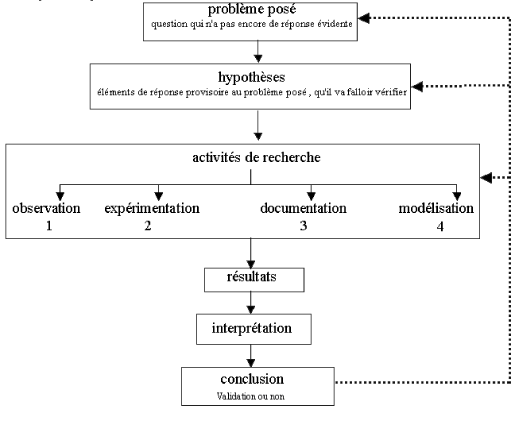
\includegraphics[width=\textwidth]{demarcheInvestigation.png}
  \caption{La démarche d’investigation (d’après Dominique Rojat, IGEN SVT)}
  \label{demarcheInvestigation}
\end{figure}
%Démarche dès la maternelle
Cette démarche serait réalisable dès la maternelle. Pour preuve, voici un extrait de l’audition de M. Georges Charpak devant la commission des affaires culturelles, familiales et sociales sur l’enseignement des disciplines scientifiques dans le primaire et le secondaire qui a eu lieu le 20~décembre 2005:
\ifthenelse{\boolean{caco}}{\begin{caco}}{\begin{quotation}}J’ai fait l’expérience d’emmener un chef d’État d’Amérique latine, en compagnie de l’ambassadeur de France, dans une classe de dernière année d’école maternelle où il a constaté qu’après trois leçons sur la densité, les élèves de cinq et six ans savaient mieux que lui, que tous les membres de son cabinet et que l’ambassadeur ce qui, d’un pamplemousse ou d’un haricot, flottait ou coulait une fois dans l’eau\dots{} Il a vu qu’ils avaient aussi appris à s’exprimer, qu’ils tenaient un cahier d’expériences. \cite[p.~157]{Rolland2006}
\ifthenelse{\boolean{caco}}{\end{caco}}{\end{quotation}}

% Littérature
Bien que cette démarche pourrait sembler plus délicate à mettre en œuvre à l’école maternelle qu’au primaire, il est possible de trouver une certaine littérature avec des projets de séquences d’enseignement. \citeA{Sacy2000} dans son livret destiné à des expériences sur l’eau et l’air en petite section précise à la page~4 qu’\og avec les connaissances de base de chacun et avec le vocabulaire des enfants, la technologie permet d’amener l’enfant à regarder autrement les objets et les éléments de sa vie quotidienne \fg{} ce qui est en accord avec la philosophie des \emph{Programmes de l’école primaire} de 1995 : \og l’enseignant-e d’école maternelle doit susciter toutes les occasions d’une découverte active du monde et de ses représentations. \fg{} \cite[p.~3]{Sacy2000}. De même, \citeA{Sanchez2012} qui ont construit 23~séquences pour des enfants du cycle~1, sont convaincus que \og à de rares exceptions près n’importe quel concept scientifique peut être abordé avec chaque enfant, à n’importe quel âge, à partir de situations adaptées \fg{} (p.~4). C’est en accord avec ce que dit \citeA[p.~8]{Coquide2002} :
\ifthenelse{\boolean{caco}}{\og}{\begin{quotation}}Si les petits ne possèdent pas encore certains types d’organisation propre à la pensée scientifique ou aux démarches technologiques, ils n’en développent pas moins une intense activité intellectuelle, nourrie par un besoin d’agir, de connaitre, de se questionner sur l’environnement qui les entoure\dots{}
\ifthenelse{\boolean{caco}}{\fg{}}{\end{quotation}}
Et en parlant de ce livre, \citeA[p.~47]{Drouard2008} précise:
\ifthenelse{\boolean{caco}}{\begin{caco}}{\begin{quotation}}Les auteurs rappellent que de vraies hypothèses propres à la méthode hypothético-déductive ne sont à envisager qu’au cycle~3 et que les \og hypothèses\fg{} ne sont pas vraiment de même nature au cycle~2. C’est pourquoi on parle dans cet ouvrage, pour la maternelle (et aussi pour le cycle~2), de situations déclenchantes et de questions inductrices, et non de situations de départ et de problèmes.
\ifthenelse{\boolean{caco}}{\end{caco}}{\end{quotation}}

% Développement du langage
Dans les \textit{Horaires et programmes d’enseignement de l’école primaire} \cite{BO2008} il est dit que l’objectif essentiel de l’école maternelle est l’acquisition d’un
langage oral riche, organisé et compréhensible par l’autre. Il existe une relation entre l’exploration du monde et le développement du langage. Selon les documents d’accompagnement des anciens programmes de 2002 \cite{Adam2005} l’exploration du monde est fondamentale et préalable à la naissance du langage. C’est une des raisons pour laquelle l’enfant doit découvrir le monde de façon active tel qu’il peut être perçu. À la fin de l’école maternelle, aucun élève ne peut avoir construit de manière stable une logique scientifique, générale et structurée. Cela n’empêche pas d’aboutir à des formulations générales et structurées à l’école maternelle.

% Le langage
En ce qui concerne le langage, \citeA{Bisault2005} a réalisé une étude sur l’argumentation dans l’enseignement des sciences en petite et moyenne section de maternelle. Il n’y a pas seulement la communication verbale qui jour un rôle dans les apprentissages, mais également les dessins, les schémas, les gestes et les actions partagées : \og Les actions et observations réalisées par quelques élèves ont été largement intégrées par les autres élèves même si elles n’ont pas toujours été systématiquement verbalisées \fg{} (p.~137).


\section{Contexte professionnel}
Cette étude est faite dans le cadre de la deuxième année du master Métiers de l’enseignement, de l’éducation et de la formation lors d’un stage d’observation et de pratique accompagnée à l’école maternelle Jean-Henri Fabre à Avignon du 7~octobre au 17~décembre~2014 et du 3~février au 20~mai~2015 dans une classe mixte de petite et moyenne section avec respectivement 19 et 7~élèves. Durant la première partie de ce stage, j’ai pu construire, mettre en œuvre et animer une séquence d’enseignement et d’apprentissage sur la germination des graines. %En 2011, l’école faisait partie du programme Écoles, collèges et lycées pour l’ambition, l’innovation et la réussite\footnote{\url{http://cache.media.education.gouv.fr/file/27/68/6/eclair_liste_etablissement_184686.pdf}}.


\section{État des lieux de la question}
% Rapport Sarmant
Selon le \emph{Rapport sur l’opération \og La main à la pâte \fg{} et l’enseignement des sciences à l’école primaire} de l’inspection générale de l’Éducation nationale \cite{Sarmant1999}, 27 classes ont été visitées du 19~mars au 4~juin 1999, réparties dans des départements fortement ou peu impliqués dans l’opération. Une différence pédagogique a été observée entre les deux types de départements : \og Les démarches pratiquées dans les classes sont nettement différentes: descriptive et affirmative dans les départements non engagés, impliquant l’activité de l’élève et sa réflexion dans les autres \fg{} (p.~5). Néanmoins, deux types de dérives ont pu être observées, la dérive du \og tout méthodologique \fg{} où l’acquisition de connaissances est un objectif mineur et la dérive du \og tout technologique \fg{} où l’activité consiste à réaliser un objet, sans autre problématique.

% Rapport IGEN
Il ne faut pas oublier, comme nous le rappelle un rapport de l’\citeA{IGEN2001} sur \textit{L’enseignement des sciences et de la technologie à l’école primaire}, que l’enseignement des sciences et de la technologie est peu pratiqué à l’école et qu’il y a très peu de classes élémentaires où cet enseignement s’appuie sur des expériences réalisées par les élèves. De plus, comme le nous remémore clairement les anciens \textit{Horaires et programmes d’enseignement de l’école primaire} \cite[p.~31]{BO2002}, il ne faut pas faire des expériences juste pour faire des expériences : 
\ifthenelse{\boolean{caco}}{\og}{\begin{quotation}}
Issue d’un questionnement provenant le plus souvent de l’activité des enfants, l’investigation menée en maternelle n’est pas conduite uniquement pour elle-même : elle débouche sur des savoir-faire et des connaissances. Même très élémentaires, ces derniers constituent un progrès important pour l’élève.
\ifthenelse{\boolean{caco}}{\fg{}}{\end{quotation}}
C’est ainsi que le document d’accompagnement \textit{Enseigner les sciences à l’école : outil pour la mise en œuvre des programmes 2002 : cycles~1 et 2} \cite{CNDP2002} a été écrit avec l’ambition d’accompagner les enseignants dans le développement d’un enseignement basé sur le questionnement et sur l’expérimentation par les élèves eux-mêmes.

% BO2008
Le 9~juin 2008, les horaires d’enseignement à l’école élémentaire par domaine disciplinaire et les programmes d’enseignement de l’école sont fixés par arrêté ministériel et sont publiés au journal officiel le 17~juin ; ce sont les \textit{Horaires et programmes d’enseignement de l’école primaire} \cite{BO2008}. À l’école maternelle, cycle des apprentissages premiers, il y a un domaine intitulé \emph{Découvrir le Monde} qui devient \emph{Découverte du monde} au cycle des apprentissages fondamentaux et \emph{Sciences expérimentales et technologie} au cycle des approfondissements. En ce qui concerne les horaires, il n’y a pas un horaire spécifique à \emph{Découvrir le Monde} en maternelle, alors qu’à l’école élémentaire la \og découverte du monde \fg{} au cycle~2 et les \og sciences expérimentales et technologie \fg{} représentent 9~\% de la durée annuelle des enseignements. %Maintenant que nous avons la place que représentent les sciences dans les sciences, on peut se demander quelle démarche est préconisée pour l’enseigner.

% Nouveaux programmes
Dans les \emph{Recommandations pour la mise en œuvre des programmes de l’école élémentaire} du \citeA{CSP2014} du 15~mai 2014, il est précisé qu’en sciences expérimentales et technologie (cycle des approfondissements), les connaissances et les compétences doivent être acquises dans le cadre d’une démarche d’investigation qui développe la curiosité, la créativité, l’esprit critique et l’intérêt pour le progrès scientifique et technique. Cependant, il n’est pas exigé que chacune des étapes de la démarche d’investigation soit systématiquement abordée lors de l’étude de chaque thème du programme. Le terme \og démarche d’investigation \fg{} n’est utilisé par le Conseil supérieur des programmes (CSP) que pour le cycle des approfondissements. Pour le cycle des apprentissages fondamentaux, le CSP ne donne aucune recommandation. Dans le \emph{Projet de programme et recommandations pour l’école maternelle} \cite{CSP2014b} du 3~juillet 2014, il est mentionné que les enfants sont conduits vers un questionnement qui s’ouvre et s’affine au fur et à mesure qu’ils agissent, essaient, constatent, formulent, représentent et réessaient. L’enseignant les aide à construire, trouver, comprendre des principes ou des généralités à travers des manipulations et des expériences. Un des objectifs est de leur donner l’habitude de regarder différemment ce qui leur paraissait auparavant familier, en devenant curieux, en s’interrogeant, en faisant des hypothèses, en comparant et contrastant. Pour la maternelle, le CSP parle d’expériences, mais pas de démarche d’investigation, ce qui n’est pas le cas du ministère de l’Éducation nationale de l’Enseignement supérieur et de la Recherche qui précise sur son site internet\footnote{\url{http://www.education.gouv.fr/cid54197/l-enseignement-des-sciences.html}} que \og dès l’école maternelle, les enfants sont initiés à la démarche d’investigation qui développe la curiosité, la créativité, l’esprit critique et l’intérêt pour le progrès scientifique et technique.\fg{} Par conséquent, on peut se demander quelle est la place de la démarche d’investigation en maternelle.

Le 26~mars 2015 est publié au Bulletin officiel de l’Éducation nationale le \textit{Programme d’enseignement de l’école maternelle} \cite{BO2015}. Selon ce programme, les enseignements sont organisés en cinq domaines d’apprentissage. Un de ses cinq domaines s’intitule \og Explorer le monde \fg{}, et il est stipulé que chaque domaine \og doit trouver sa place dans l’organisation du temps quotidien \fg{}. Le domaine \og Explorer le monde \fg{} se définit en deux sous-domaines : \og Se repérer dans le temps et l’espace \fg{} et \og Explorer le monde du vivant, des objets et de la matière \fg{} où il est précisé que \og l’enseignant propose des activités qui amènent les enfants à observer, formuler des interrogations plus rationnelles, construire des relations entre les phénomènes observés, prévoir des conséquences, identifier des caractéristiques susceptibles d’être catégorisées \fg{} afin de \og les aider à découvrir, organiser et comprendre le monde qui les entoure \fg{}. Bien que la démarche d’investigation ne soit pas spécifiée, elle répond aux exigences du programme.

Pour finir, bien qu’il ne s’agisse pas d’un document spécifique à la maternelle, on remarque que la démarche d’investigation fait partie du tout nouveau \emph{Socle commun de connaissances, de compétences et de culture} \cite{Socle2015} où l’élève doit découvrir la nature environnante par une approche scientifique qui est fondée sur l’observation, la manipulation et l’expérimentation.

\section{Intérêt de la question}
Les \textit{Horaires et programmes d’enseignement de l’école primaire} \cite{BO2008} parlent de démarche d’investigation, en générale et plus précisément pour le cycle~3. La recommandation du ministère de l’Éducation nationale, de l’Enseignement supérieur et de la Recherche est que les enfants soient initiés à cette démarche dès la maternelle. Dans quelle mesure l’enseignement de cette démarche se fait-il en maternelle ? La réponse à cette question pourra permettre un premier état des lieux des pratiques enseignantes, ce qui peut donner des repères aux (jeunes) enseignants de maternelle.
	\ifthenelse{\boolean{papier}}{\clearemptydoublepage}{}
\chapter{Problématique}
\section{Question envisagée en rapport avec la profession}\label{question}
La démarche d’investigation (cf. figure p.~\pageref{demarcheSci} de l’annexe~\ref{questionnaireWeb}), utilisée par les chercheurs, a été adaptée pour l’enseignement des sciences à l’école élémentaire et pour les années postérieures. La littérature nous montre l’existence de certaines dérives. En effectuant une enquête des pratiques enseignantes à partir d’un questionnaire, nous allons essayer faire le point sur la pratique enseignante lors de la mise en œuvre de la démarche d’investigation en maternelle. La question qui se pose est : \og Dans quelle mesure l’enseignement des sciences par la démarche d’investigation est-il envisageable en maternelle ? \fg{} 

Gauthier et al. (1986, cité dans \citeA[p.~23]{Long2004}) considèrent qu’\og un problème de recherche est considéré comme étant un écart ou un manque à combler dans le domaine de nos connaissances entre ce que nous savons et ce que nous devrions ou désirons savoir sur le réel. \fg{} Nous sommes conscients qu’il ne s’agit pas d’une question de recherche, puisqu’il n’y a pas d’\og écart \fg{}, il s’agit plus d’un état des lieux!% qui devrait permettre justement à mesurer cet écart. Ce qui pourrait déboucher sur une question de recherche.

\section{Réponses possibles}
À la question \og Dans quelle mesure l’enseignement des sciences par la démarche d’investigation est-il envisageable en maternelle ? \fg{} plusieurs réponses sont possibles :
\begin{itemize}
\item Les sciences ne sont pas enseignées.
\item Les sciences sont enseignées, mais pas en utilisant la démarche d’investigation.
\item Les sciences sont enseignées, en utilisant la démarche d’investigation.
\end{itemize}

Dans ces deux derniers cas, nous allons regarder plus précisément la démarche mise en place et comparer la position des enseignants aux différentes assertions que nous avons trouvées dans la littérature. Notamment l’affirmation de \citeA[p.~4]{Sanchez2012} : \og à de rares exceptions près n’importe quel concept scientifique peut être abordé avec chaque enfant, à n’importe quel âge, à partir de situations adaptées \fg{}, ainsi que la dérive du \og tout méthodologique \fg{} et la dérive du \og tout technologique \fg{} misent en avant par \citeA{Sarmant1999}. Nous allons également comparer les heures d’enseignement des sciences aux heures qui sont censées être enseignées au cycle~2 et voir comment la démarche d’investigation est adaptée.

De la même manière que nous avons remarqué à la section \ref{question} qu’il ne s’agissait pas d’une question de recherche, nous remarquerons qu’ici nous ne sommes pas en présence d’une série d’hypothèses envisageables, mais simplement d’un choix de réponses possibles !	
	\ifthenelse{\boolean{papier}}{\clearemptydoublepage}{}
\chapter{Étude}
\section{Descriptif du dispositif}
Lors de la première partie du stage qui s’est déroulé d’octobre à décembre~2014, j’ai pu mettre en œuvre une partie d’une séquence d’enseignement en sciences en petite et moyenne section de maternelle. Cela m’a permis de me rendre compte de ce qu’il est possible et impossible de faire. Afin d’avoir une représentation plus précise de ce qu’il est possible de faire, j’ai préféré orienter mon étude à la pratique enseignante d’une manière générale, d’où l’idée du questionnaire. L’étude sera faite à partir d’un questionnaire qui permet de valider différentes affirmations exposées dans la section~\ref{cadre}, \og Cadre de l’étude \fg{} (p.~\pageref{cadre}).

\section{Mode de recueil de données}
L’étude se déroulera en deux étapes. La première étape correspond au questionnaire papier (cf. annexe~\ref{questionnairePapier}, p.~\pageref{questionnairePapier}) qui a été distribué à l’école maternelle Jean-Henri Fabre d’Avignon le 23~avril 2015 et qui a été rempli par six enseignantes. Cette étape m’a permis de tester le questionnaire et de modifier certaine question, principalement la question~4 : \og Enseignez-vous seulement en maternelle ? \fg{} qui a été remplacée par \og Enseignez-vous également au cycle~2 ou au cycle~3 ? \fg{} En effet, un professeur des écoles maitre formateur qui enseigne en maternelle et à l’université répondra \og non \fg{} à la première question, alors que l’objectif de la question était de savoir s’il enseigne à d’autres classes du primaire.

La deuxième étape correspond à un questionnaire web qui a été rempli par 67~enseignantes ou enseignants de maternelle du 25~avril au 4~mai 2015. C’est ce deuxième questionnaire qui se trouve à l’annexe~\ref{questionnaireWeb} (p.~\pageref{questionnaireWeb}) que nous allons analyser.

\section{Mode de traitement des données recueillies}
Les données sont récupérées dans une feuille de calcul exploitable par un tableur. Il s’agit essentiellement de questions fermées et de variables qualitatives. Il existe des logiciels d'analyse statistique. Malheureusement, par manque de connaissance et de temps, la possibilité d’utiliser PSPP une alternative libre à SPSS ne sera pas abordée. Le traitement des données recueillies prendra la forme d’une simple analyse statistique ainsi que de tableaux croisés.
	\ifthenelse{\boolean{papier}}{\clearemptydoublepage}{}
\chapter{Analyse}
\section{Description du questionnaire}
Le questionnaire contient 21~questions obligatoires à choix multiples et 3~zones facultatives de texte libre. Avant d’analyser le questionnaire, voici une description succincte des 12~pages du questionnaire :
\begin{description}
\item[Page 1 : La démarche d’investigation en maternelle] Présentation du questionnaire et de son objectif.
\item[Page 2 : Population cible] Question vérifiant que la personne appartient bien à la population ciblée.
\item[Page 3 : Mise au point] Lien vers deux images détaillant la démarche d’investigation.
\item[Page 4 : Cadre] Questions par rapport à des variables qui peuvent influencer l’ensemble du questionnaire (nombre d’années d’expérience\dots)
\item[Page 5 : Enseignement des sciences] Questions sur la position de l’enseignant par rapport aux sciences. Pour les enseignants qui sont dans une classe où les sciences ne sont pas enseignées, le questionnaire se poursuit à la page~9  et pour les enseignants qui sont déchargés de l’enseignement des sciences le questionnaire se poursuit à la page~11.
\item[Page 6 : Démarche] Première série de questions sur les démarches mises en œuvre lors de l’enseignement des sciences. Pour les enseignants qui n’utilisent jamais la démarche d’investigation, le questionnaire se poursuit à la page~10 et il se poursuit à la page~11 pour ceux et celles qui ne répondent pas à la question sur la fréquence d’utilisation de la démarche d’investigation.
\item[Page 7 : Démarche d’investigation] Questions sur la démarche d’investigation.
\item[Page 8 : Activités de recherche] Quelles sont les différentes activités mises en place lors de la phase d’investigation ?
\item[Page 9] Zone facultative de texte libre pour permettre d’expliquer pourquoi les sciences ne sont pas enseignées.
\item[Page 10] Zone facultative de texte libre pour permettre d’expliquer pourquoi la démarche d’investigation n’est pas utilisée.
\item[Page 11] Zone facultative de texte libre afin de pouvoir ajouter des commentaires.
\item[Page 12] Page de remerciement.
\end{description}

\section{Présentation du questionnaire et de son objectif}
Le texte de cette première page du questionnaire est : \og Dans le cadre du master Métiers de l’enseignement, de l’éducation et de la formation, je rédige un mémoire professionnel ayant pour objectif de mieux connaitre la pratique enseignante par rapport à la démarche d’investigation. Ce questionnaire contient au maximum 21~questions, majoritairement fermées, ainsi qu’une zone finale de commentaires. Merci de votre participation. \fg{} L’objectif du questionnaire devait être clair afin que les enseignants interrogés puissent être dans une démarche réflexive.

\section{Population cible}
Le texte de cette première question est : \og Êtes-vous enseignante ou enseignant en maternelle dans une école appliquant les programmes du ministère français de l’Éducation nationale ? (Que cela soit en France ou à l’étranger.) \fg{} Le but était d’inclure non seulement les départements et régions d’outre-mer et collectivités d’outre-mer, mais également les écoles membres de l’Agence pour l’enseignement français à l’étranger. Soixante-quinze personnes ont répondu au questionnaire, dont sept n’appartenant pas à la population ciblée. L’effectif pris en compte pour le reste du questionnaire sera donc de 68~enseignants.

\section{Mise au point}
Lors du passage du premier questionnaire dont le titre était \og La démarche d’investigation en maternelle \fg{}, une des enseignantes s’est demandé ce que c’était la démarche d’investigation. Par la suite, lorsqu’elle a vu la figure sur la démarche d’investigation (page~4 du questionnaire de l’annexe~\ref{questionnairePapier}) elle a associé la démarche d’investigation à la démarche scientifique. Afin que le concept de démarche d’investigation soit le plus explicite, j’ai décidé de mettre un lien vers deux images représentant la démarche d’investigation (cf. figures du questionnaire de l’annexe~\ref{questionnaireWeb}) : une représentation avec des pictogrammes exploitable en maternelle et un schéma montrant la différence entre la démarche d’investigation et la démarche scientifique.

\section{Cadre}
La deuxième question (\og Depuis combien d’années enseignez-vous en maternelle ? \fg{}) permet de connaitre l’expérience de l’enseignant (Moins de 5~ans, Entre 5 et 10~ans, Plus de 10~ans). Cette variable sera utilisée lors de l’analyse d’autres questions. La moitié (34/68) des personnes qui ont répondu à cette question ont moins de 5~années d’expérience, ce qui peut s’expliquer par le fait que la promotion de ce questionnaire a été faite entre autres dans des groupes de professeurs des écoles stagiaires.

La troisième question concerne la durée moyenne hebdomadaire d’enseignement des sciences en maternelle que nous allons comparer au nombre d’heures d’enseignement censées être consacrées à la \og Découverte du monde \fg{} qui est en moyenne 2~h~15 par semaine selon les horaires de l’école élémentaire d’après le Bulletin officiel de 2008. Une très grande majorité des enseignants de maternelle (46/60) enseigne les sciences moins de deux heures par semaines, par contre il y a deux fois plus d’enseignants (30/46) qui font entre une et deux heures que moins d’une heure (16/46). Parmi ces seize enseignants, cinq n’enseignent pas les sciences : pour trois d’entre eux c’est quelqu’un d’autre qui s’en charge et pour les deux autres font partie de classe où les sciences ne sont pas enseignées, soit en tant qu’enseignant ou enseignante unique soit en tant que modulateur ou modulatrice.

La question suivante (\og Enseignez-vous également au cycle~2 ou au cycle~3 ? \fg{}) était destinée à voir s’il y avait une différence entre ceux et celles qui n’enseignent quand maternelle et ceux et celles qui enseignent sur plusieurs cycles. Cinquante-huit des enseignants n’exercent pas aux cycles~2 et 3. À première vue, il n’y aurait pas point commun pour les neuf autres personnes.

En ce qui concerne le nombre de classes enseignées (\og À combien de classes enseignez-vous en maternelle ? \fg{}), il s’agit surtout d’enseignants qui ont en charge la classe à plein temps (28/68) ou à mi-temps (20/68). En comparant cette variable avec d’autres critères, il n’y rien de significatif.

La dernière question (\og En quelle section enseignez-vous ? \fg{}) de cette section devait être une question à choix multiples où les enseignants devaient de prendre en compte pour cette question ainsi que pour le reste du questionnaire, seulement la classe ou le niveau où votre enseignement des sciences est le plus significatif. Seulement un peu plus de la moitié des classes (35/68) sont des classes à un seul niveau.

\section{Enseignement des sciences}
La première question de cette section est une question d’autoévaluation des enseignants par rapport à leur engagement dans l’enseignement des sciences. Une très forte majorité (52/68) se considère comme une personne engagée ou très engagée. Par contre, six enseignants ne se considèrent pas du tout engagés, deux d’entre eux font partie de classes où les sciences ne sont pas enseignées, et pour les quatre autres c’est quelqu’un d’autre qui s’en charge.

Ensuite, j’ai voulu tester leur position par rapport à l’affirmation \og À de rares exceptions près n’importe quel concept scientifique peut être abordé avec chaque enfant, à n’importe quel âge, à partir de situations adaptées \fg{} qu’on trouve dans \textit{Sciences à vivre : 23 séquences pour découvrir le monde du vivant et de la terre avec des enfants du cycle 1} de \citeA{Sanchez2012}. Les enseignants sont d’accord à plus de 80~\% avec cette assertion, et plus précisément 49~\% (33/68) sont plutôt d’accord et 32~\% (22/68) sont totalement d’accord.

Le but de la question suivante (\og Il est possible d’enseigner les sciences en maternelle en utilisant la démarche d’investigation. \fg{}) était de connaitre la prédisposition des enseignants par rapport à la démarche d’investigation. Il y plus de personnes qui sont en accord avec cette affirmation qu’avec l’affirmation précédente, 54~\% qui sont totalement d’accord et 38~\% qui sont plutôt d’accord.

La section suivant est destinée seulement à ceux qui enseignent les sciences, d’où l’intérêt de cette question (\og Enseignez-vous les sciences dans votre classe de maternelle ? \fg{}). Soixante personnes ont répondu par l’affirmative, ce qui sera l’effectif de référence pour la partie suivante du questionnaire.

\section{Démarche d’investigation}
La première série de questions, page~6 du questionnaire, ne fait pas spécifiquement référence à la démarche d’investigation, ce qui n’est pas le cas des deux questions de la page~7 du questionnaire.

La question \og Faites-vous des apports théoriques avant les expériences ? \fg{} a pour objectif d’être comparée à \og Adoptez-vous la démarche d’investigation lors de vos séances de sciences ? \fg{} L’idée de l’enseignement par la démarche d’investigation est d’apporter un apport théorique par l’investigation. Y a-t-il une relation entre les réponses entre ces deux questions, dont les réponses sont retranscrites à la table~\ref{theorie}.
\begin{table}[h!btp]
\centering
\caption{\label{theorie} Apports théoriques / Démarche d’investigation}
	\begin{tabular}{|c|c|c|c|c|}
	\cline{2-5}
	\multicolumn{1}{c|}{} & \multicolumn{4}{c|}{Adoptez-vous la démarche d’investigation?} \\ 
	\hline 
	\begin{minipage}[l]{3.7cm}\begin{flushleft}Faites-vous des apports théoriques avant les expériences ?\end{flushleft}\end{minipage} & Jamais & \begin{minipage}[c]{2cm}Occasion- nellement\end{minipage} & Souvent & Toujours \\ 
	\hline 
	Jamais & 1 & 5 & 9 & 7 \\ 
	\hline 
	Occasionnellement & 1 & 4 & 17 & 6 \\ 
	\hline 
	Souvent & 0 & 1 & 3 & 3 \\ 
	\hline 
	Toujours & 0 & 0 & 0 & 3 \\ 
	\hline 
	\end{tabular}
\end{table}
Le test du $\chi^2$ permet de savoir si les deux variables sont indépendantes. Pour ces données, nous avons $\chi^2=9,8$ qui est inférieur au seuil de référence $\chi^2_{9;0,05}=16,9$. Les deux variables sont indépendantes.

La question suivante est : \og Faites-vous des expériences sans questionnement initial ? \fg{} On a les données de la table~\ref{questionnement}.
\begin{table}[h!btp]
\centering
\caption{\label{questionnement} Questionnement initial / Démarche d’investigation}
	\begin{tabular}{|c|c|c|c|c|}
	\cline{2-5}
	\multicolumn{1}{c|}{} & \multicolumn{4}{c|}{Adoptez-vous la démarche d’investigation?} \\ 
	\hline 
	\begin{minipage}[l]{3.7cm}\begin{flushleft}Faites-vous des expériences sans questionnement initial ?\end{flushleft}\end{minipage} & Jamais & \begin{minipage}[c]{2cm}Occasion- nellement\end{minipage} & Souvent & Toujours \\ 
	\hline 
	Jamais & 0 & 2 & 12 & 13 \\ 
	\hline 
	Occasionnellement & 1 & 6 & 12 & 4 \\ 
	\hline 
	Souvent & 1 & 2 & 5 & 1 \\ 
	\hline 
	Toujours & 0 & 0 & 0 & 1 \\ 
	\hline 
	\end{tabular}
\end{table}
$\chi^2=12,8$, ce qui reste inférieur à $\chi^2_{9;0,05}$. Les deux variables sont indépendantes.

La question suivante, \og Faites-vous des activités exclusivement technologiques, c’est-à-dire de réaliser un objet sans autre problématique. \fg{}, correspond à la dérive du \og tout technologique \fg{} observée par \citeA{Sarmant1999}. Et on obtient les données  de la table~\ref{technologiques}.
\begin{table}[h!btp]
\centering
\caption{\label{technologiques} Activités technologiques / Démarche d’investigation}
	\begin{tabular}{|c|c|c|c|c|}
	\cline{2-5}
	\multicolumn{1}{c|}{} & \multicolumn{4}{c|}{Adoptez-vous la démarche d’investigation?} \\ 
	\hline 
	\begin{minipage}[l]{3.7cm}\begin{flushleft}Faites-vous des activités exclusivement technologiques ?\end{flushleft}\end{minipage} & Jamais & \begin{minipage}[c]{2cm}Occasion- nellement\end{minipage} & Souvent & Toujours \\ 
	\hline 
	Jamais & 0 & 3 & 11 & 9 \\ 
	\hline 
	Occasionnellement & 1 & 6 & 14 & 9 \\ 
	\hline 
	Souvent & 1 & 0 & 2 & 0 \\ 
	\hline 
	Toujours & 0 & 0 & 0 & 1 \\ 
	\hline 
	\end{tabular}
\end{table}
Cette fois-ci $\chi^2=12,9$, ce qui est également inférieur à $\chi^2_{9;0,05}$. Par conséquent, les deux variables sont indépendantes. On remarquera que 38~\% des enseignants (23/60) ne font jamais des activités exclusivement technologiques, et 50~\% (30/60) le font occasionnellement.

La dernière question de la page~6 (\og Adoptez-vous la démarche d’investigation lors de vos séances de sciences ? \fg{} ) est un filtre. Les questions suivantes font spécifiquement référence à cette démarche. Quarante-huit personnes sur  soixante qui enseignent les sciences déclarent l’utiliser souvent (29/60) ou toujours (19/60), ce qui représente 80~\% de ceux qui enseignent la science. Deux personnes déclarent ne jamais l’utiliser, l’effectif pour les questions suivantes ne sera plus de soixante, mais de cinquante-huit.

La première question spécifique à la démarche d’investigation concerne la deuxième dérive signalée par \citeA{Sarmant1999}, la dérive du \og tout méthodologique \fg{}. Cinquante-trois pour cent (31/58) des enseignants qui enseignent les sciences en maternelle privilégient souvent la démarche d’investigation à l’acquisition des connaissances et 19~\% (11/58) la privilégient toujours.

Une autre question concernant la démarche d’investigation était sur l’adaptation de la démarche d’investigation. L’intitulé de la question était : \og Adaptez-vous la démarche d’investigation en formulant vous-même la question problématique plutôt que de construire progressivement en classe le problème à partir d’un étonnement, d’une curiosité ou d’un questionnement ? \fg{} La majorité, soit 53~\% (31/58) le font occasionnellement et 26~\% (15/58) souvent.

La dernière série de questions concerne les différents types d’investigation pour les activités de recherche (cf. fig.~\ref{demarcheInvestigation} p.~\pageref{demarcheInvestigation}). Il fallait compléter la phrase suivante : \og Lorsque vous utilisez la démarche d’investigation, les activités de recherche réalisées par les élèves s’appuient sur\dots{} \fg{} Si l’on comptabilise les individus qui ont répondu par \og Toujours \fg{} ou \og Souvent \fg{}, on a :
\begin{itemize}
\item 67~\% (39/58) pour divers essais dont les résultats sont comparés (tâtonnement expérimental) ;
\item 55~\% (32/58) pour une observation directe ou assistée par un instrument (qui ne soit pas l’ordinateur) ou sur l’exploitation de documents (images, données, résultats d’expériences) ;
\item 47~\% (27/58) pour un dispositif où un seul facteur varie et où les résultats sont recueillis par l’observation ou la mesure (expérimentation directe ;
\item 36~\% (21/58) pour une réalisation matérielle (construction d’un objet, d’un modèle, recherche d’une solution technique) ;
\item 22~\% (13/58) pour la lecture de documents papier ou électroniques ou par l’interview de personnes compétentes (recherche documentaire).
\end{itemize}
	\ifthenelse{\boolean{papier}}{\clearemptydoublepage}{}
\chapter{Conclusion}
La question initiale était de savoir dans quelle mesure l’enseignement des sciences par la démarche d’investigation était envisageable en maternelle, de savoir si les sciences sont enseignées et si la démarche d’investigation est utilisée.

Un questionnaire a été soumis à 68~enseignants. Une très forte majorité (93~\%) d’entre eux pensent qu’il est possible d’enseigner les sciences en maternelle en utilisant la démarche d’investigation. Par contre 84~\% des enseignants qui adoptent la démarche d’investigation privilégient la démarche à l’acquisition des connaissances.
	% Épilogue
	\bibliographystyle{plain-fr}
\nocite{Lamarque2006}
\bibliography{../commun/ESPE}
%\bibliography{commun/ESPE}
	\appendix
	\ifthenelse{\boolean{papier}}{\clearemptydoublepage}{}
\chapter{Questionnaire papier}
\label{questionnairePapier}
Questionnaire initial qui a été testé à l’école maternelle Jean-Henri Fabre d’Avignon.


\ifthenelse{\boolean{caco}}{%
	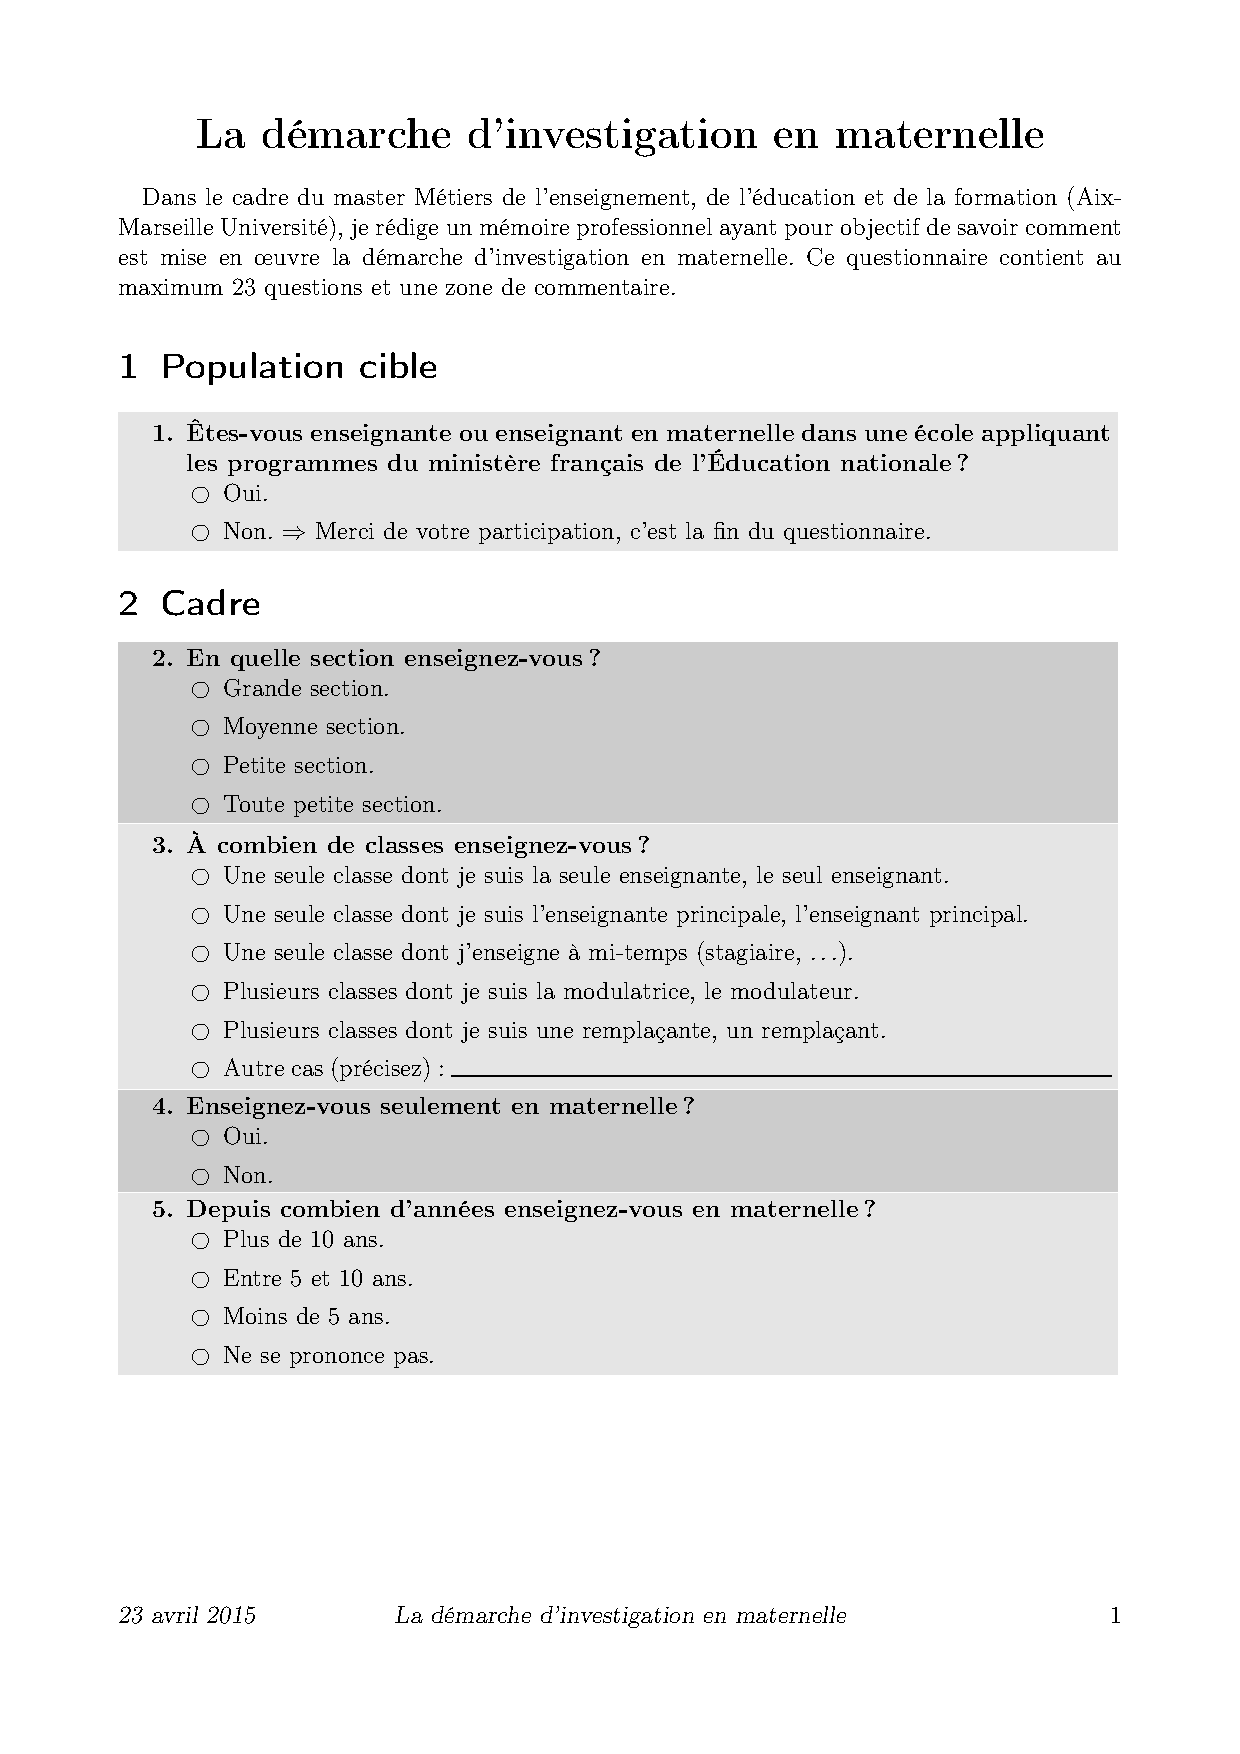
\includepdf[pages=-,pagecommand=\thispagestyle{plain},scale=0.7,frame=true,offset=15 0]{tex/questionnaire_2015-04-23.pdf}
}{%
	\ifthenelse{\boolean{papier}}{%	
		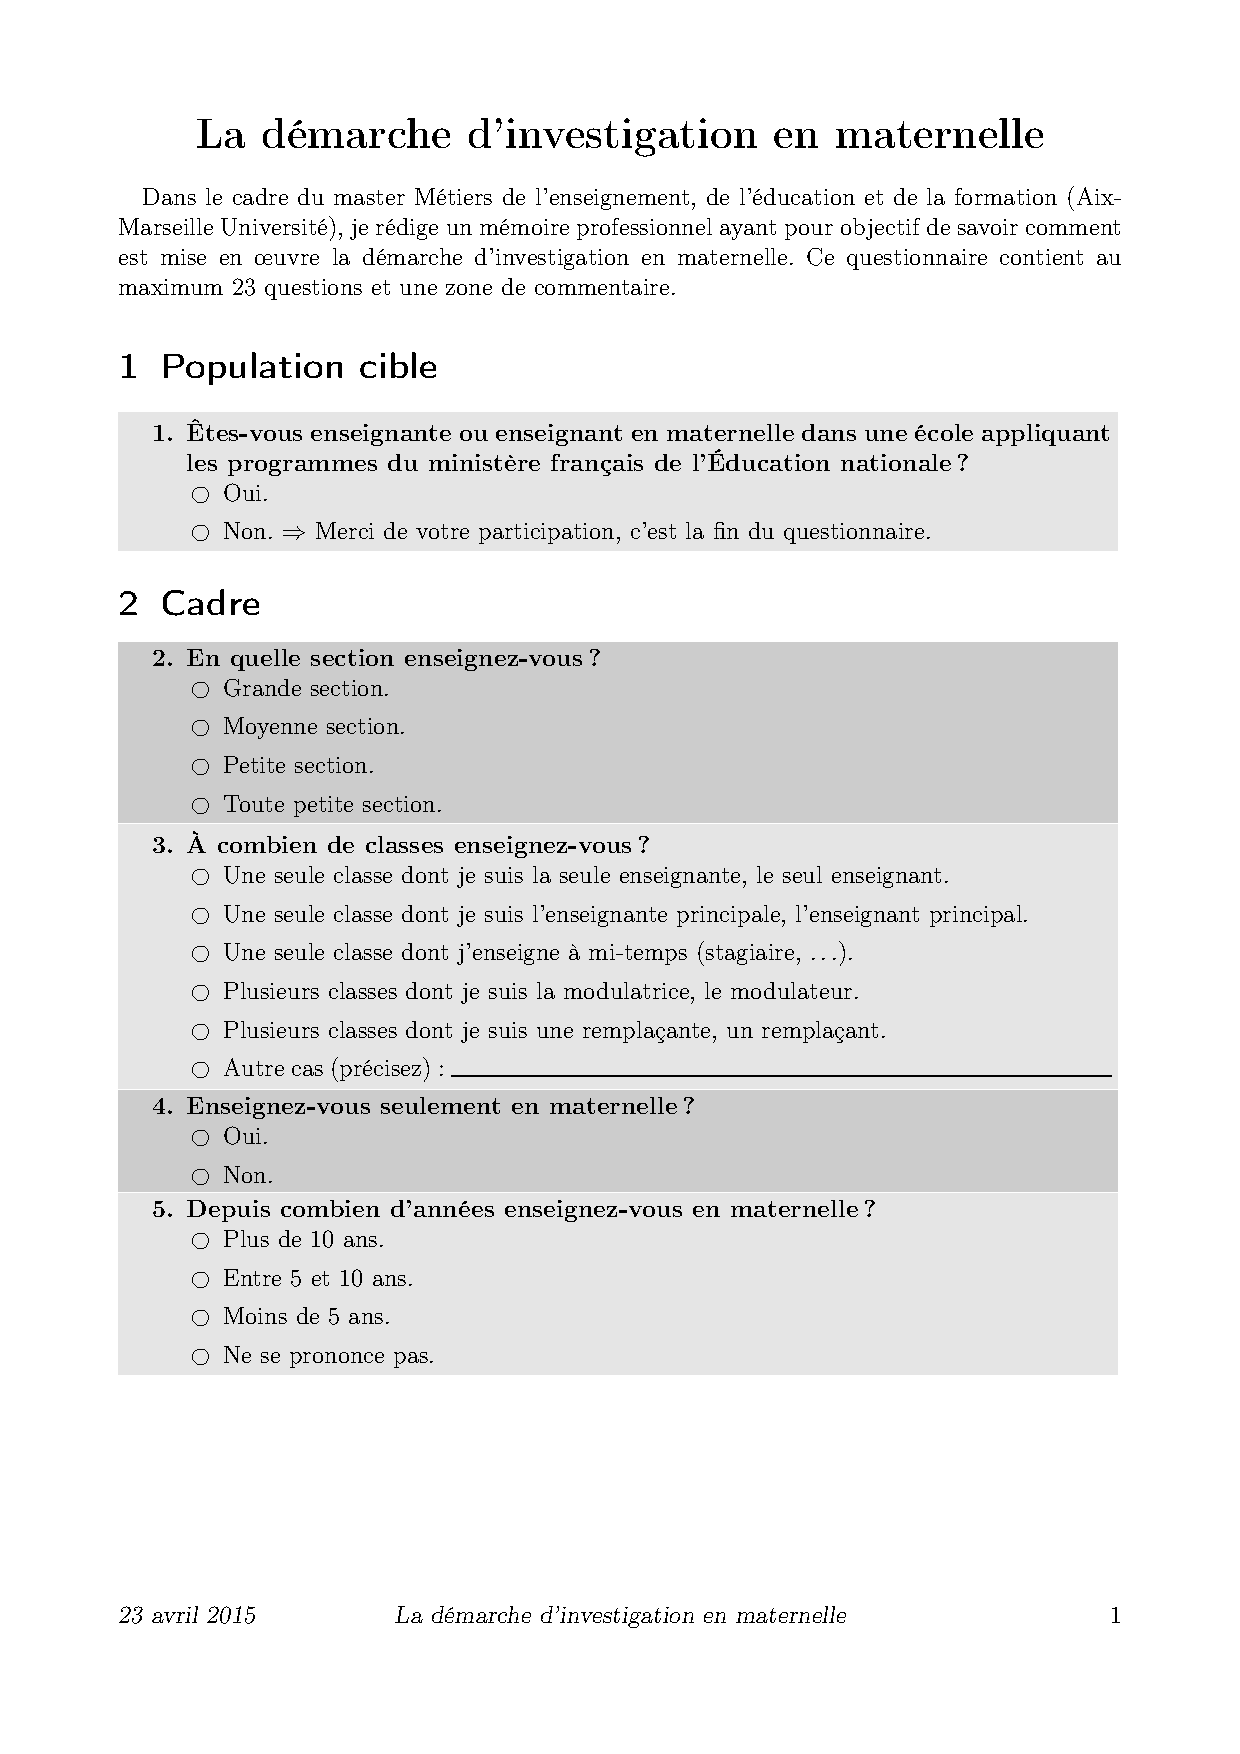
\includepdf[pages=-,pagecommand=\thispagestyle{plain},scale=0.61,frame=true,offset=-29 50]{tex/questionnaire_2015-04-23.pdf}		
	}{%
		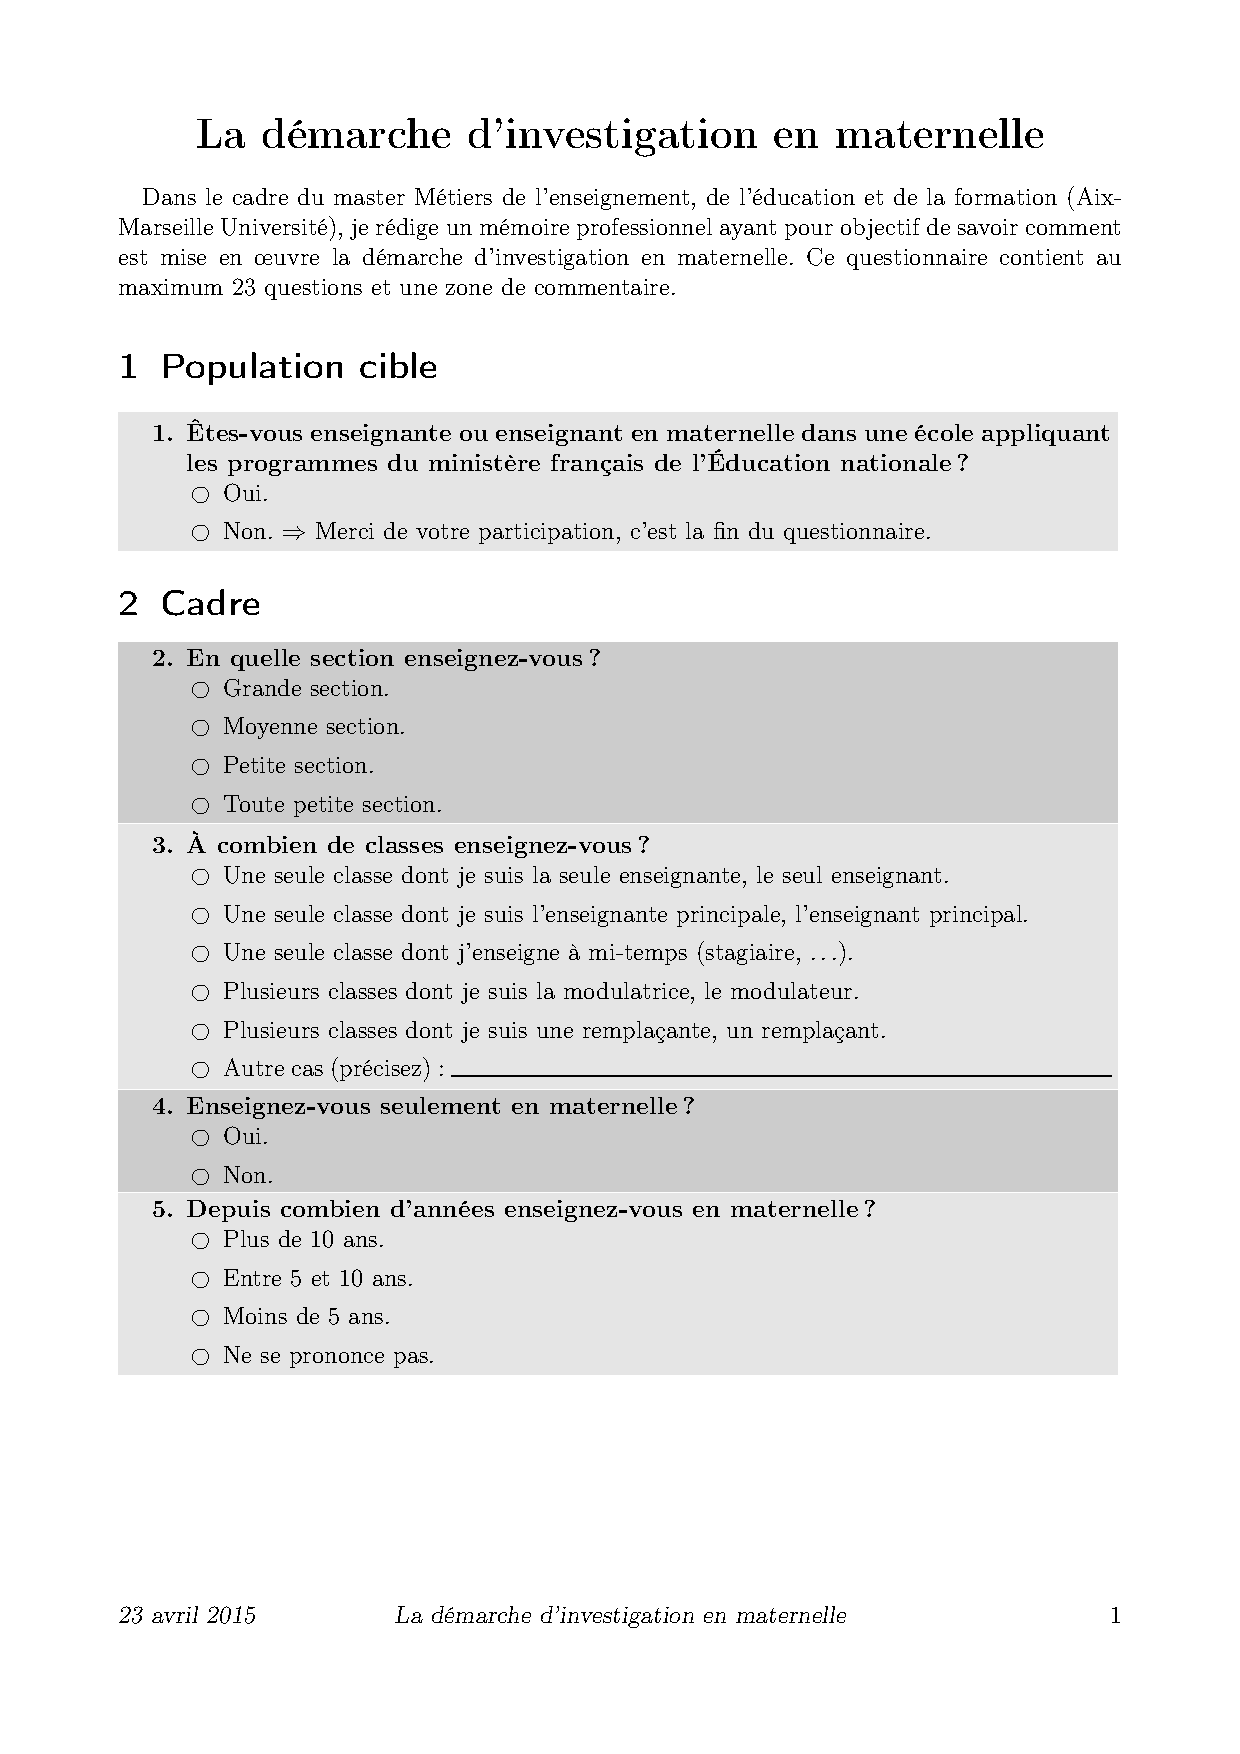
\includepdf[pages=-,pagecommand=\thispagestyle{plain},scale=0.67,frame=true,offset=0 40]{tex/questionnaire_2015-04-23.pdf}
	}
}


\ifthenelse{\boolean{papier}}{\clearemptydoublepage}{}
\chapter{Questionnaire en ligne}
\label{questionnaireWeb}
Version texte du questionnaire en ligne réalisé en utilisant Google Forms. Ce questionnaire au format texte était utilisable par les personnes ne désirant pas utiliser le formulaire Google. Il est suivi de deux images de la démarche d’investigation auxquelles le questionnaire fait référence aux lignes~28 et 29.

\ifthenelse{\boolean{caco}}{%
	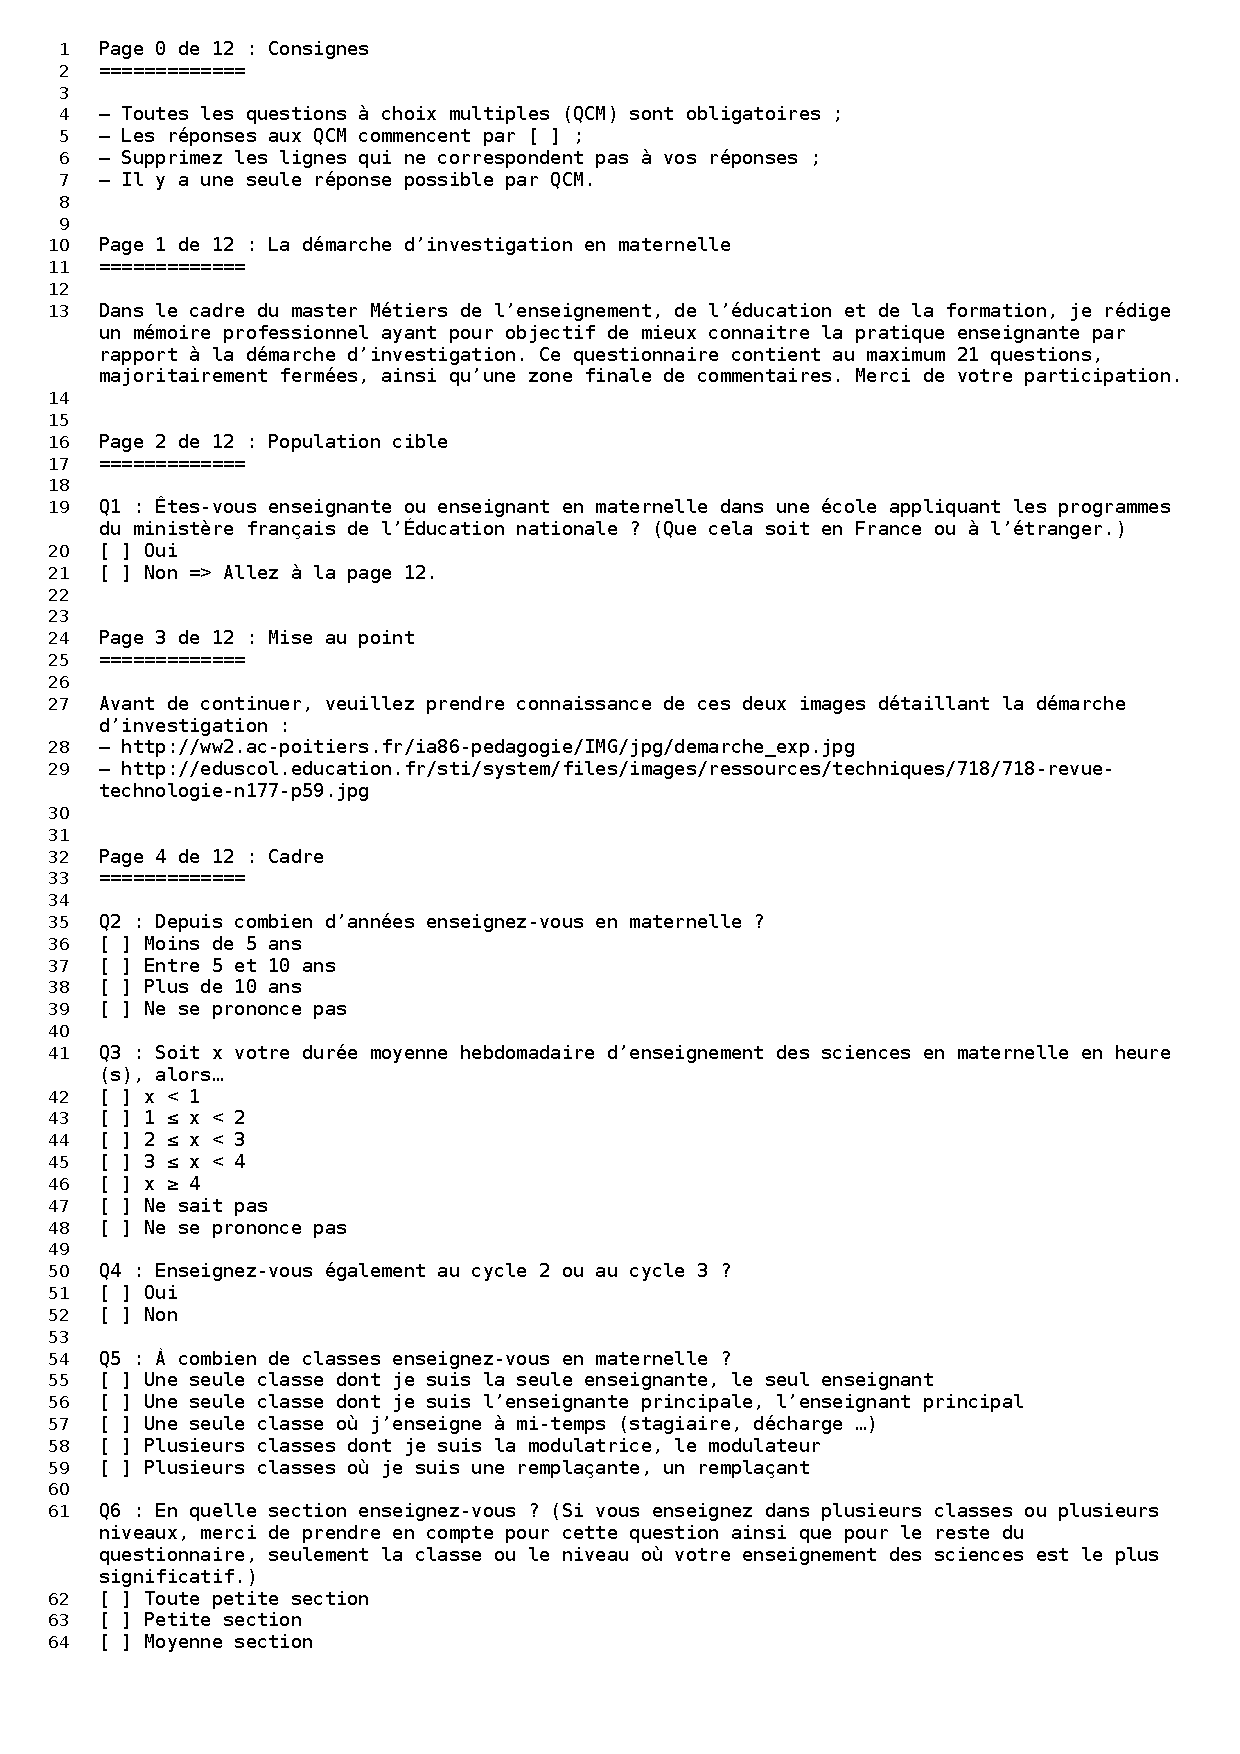
\includepdf[pages=-,pagecommand=\thispagestyle{plain},scale=0.7,frame=true,offset=15 0]{www/questionnaire}
}{%
	\ifthenelse{\boolean{papier}}{%	
		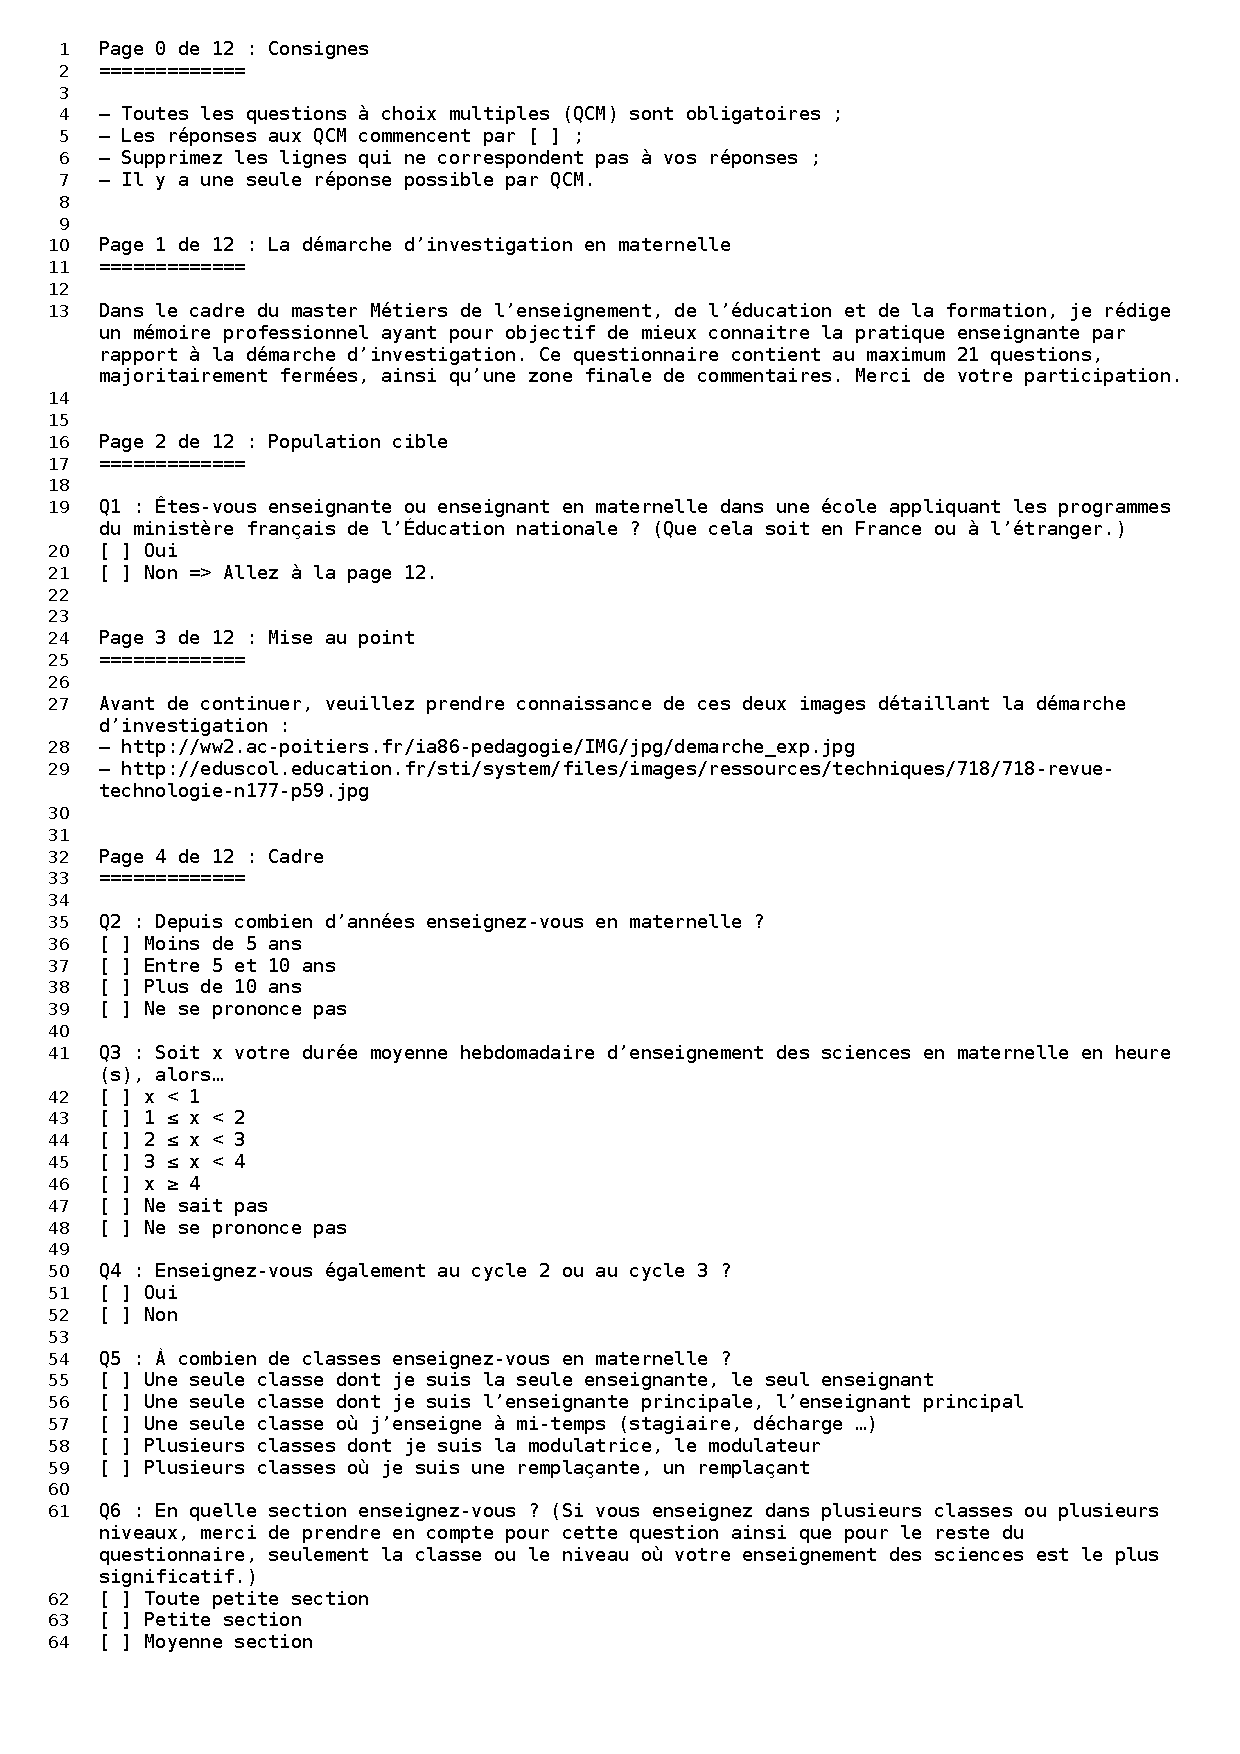
\includepdf[pages=-,pagecommand=\thispagestyle{plain},scale=0.61,frame=true,offset=-29 50]{www/questionnaire}
	}{%
		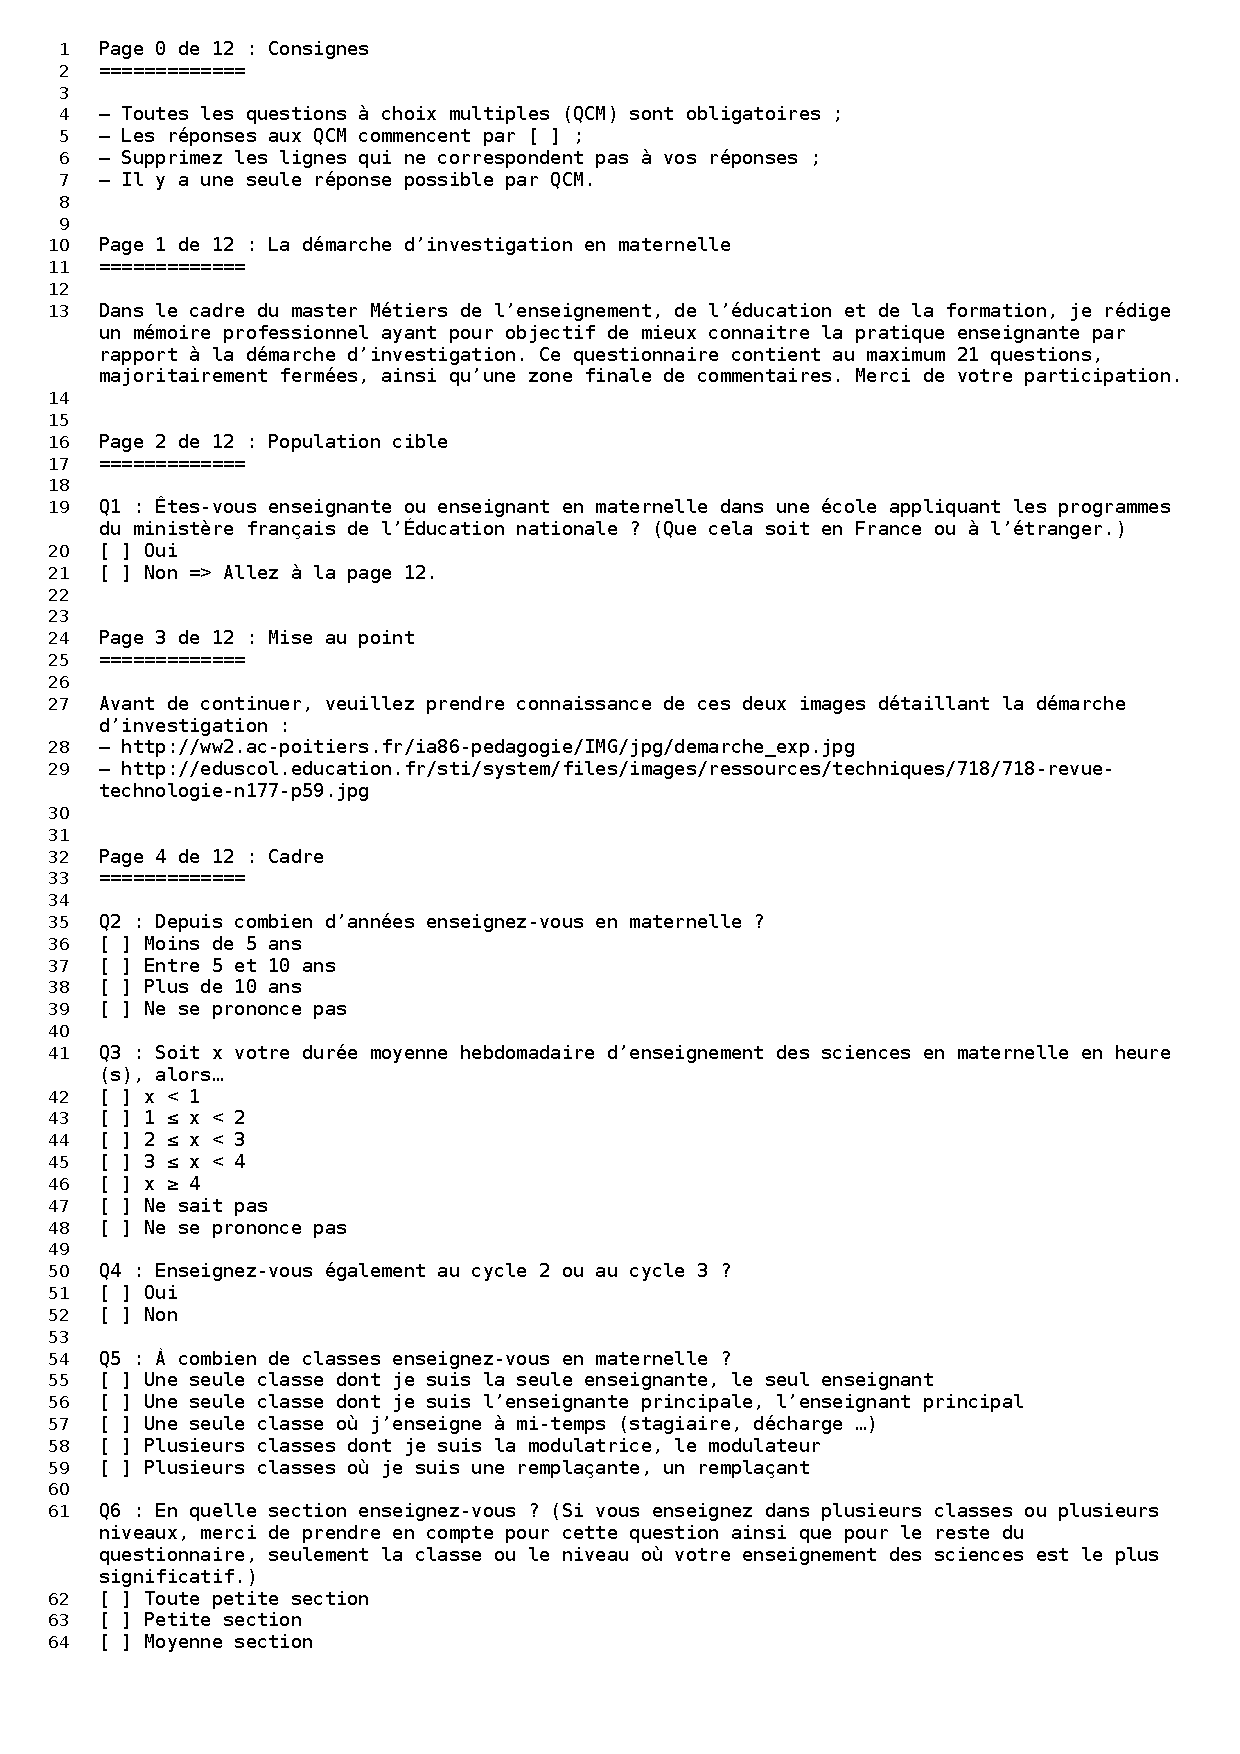
\includepdf[pages=-,pagecommand=\thispagestyle{plain},scale=0.67,frame=true,offset=0 40]{www/questionnaire}
	}
}

\mbox{}
\vfill
\noindent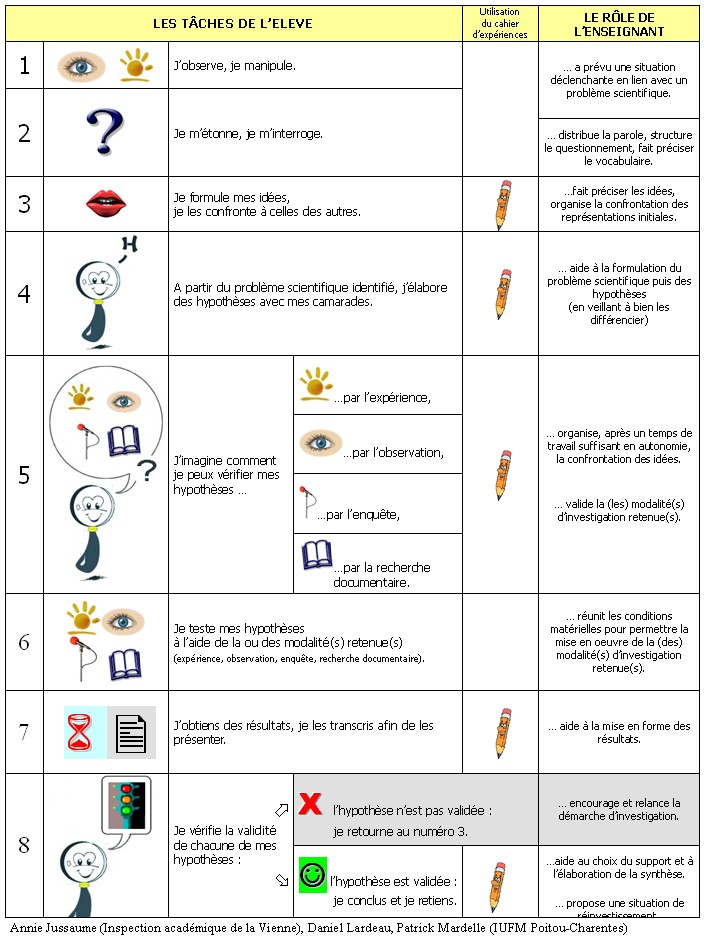
\includegraphics[width=\textwidth]{demarche_exp}
\vfill
\newpage

\ifthenelse{\boolean{caco}}{%
	\mbox{}
	\vfill
	\noindent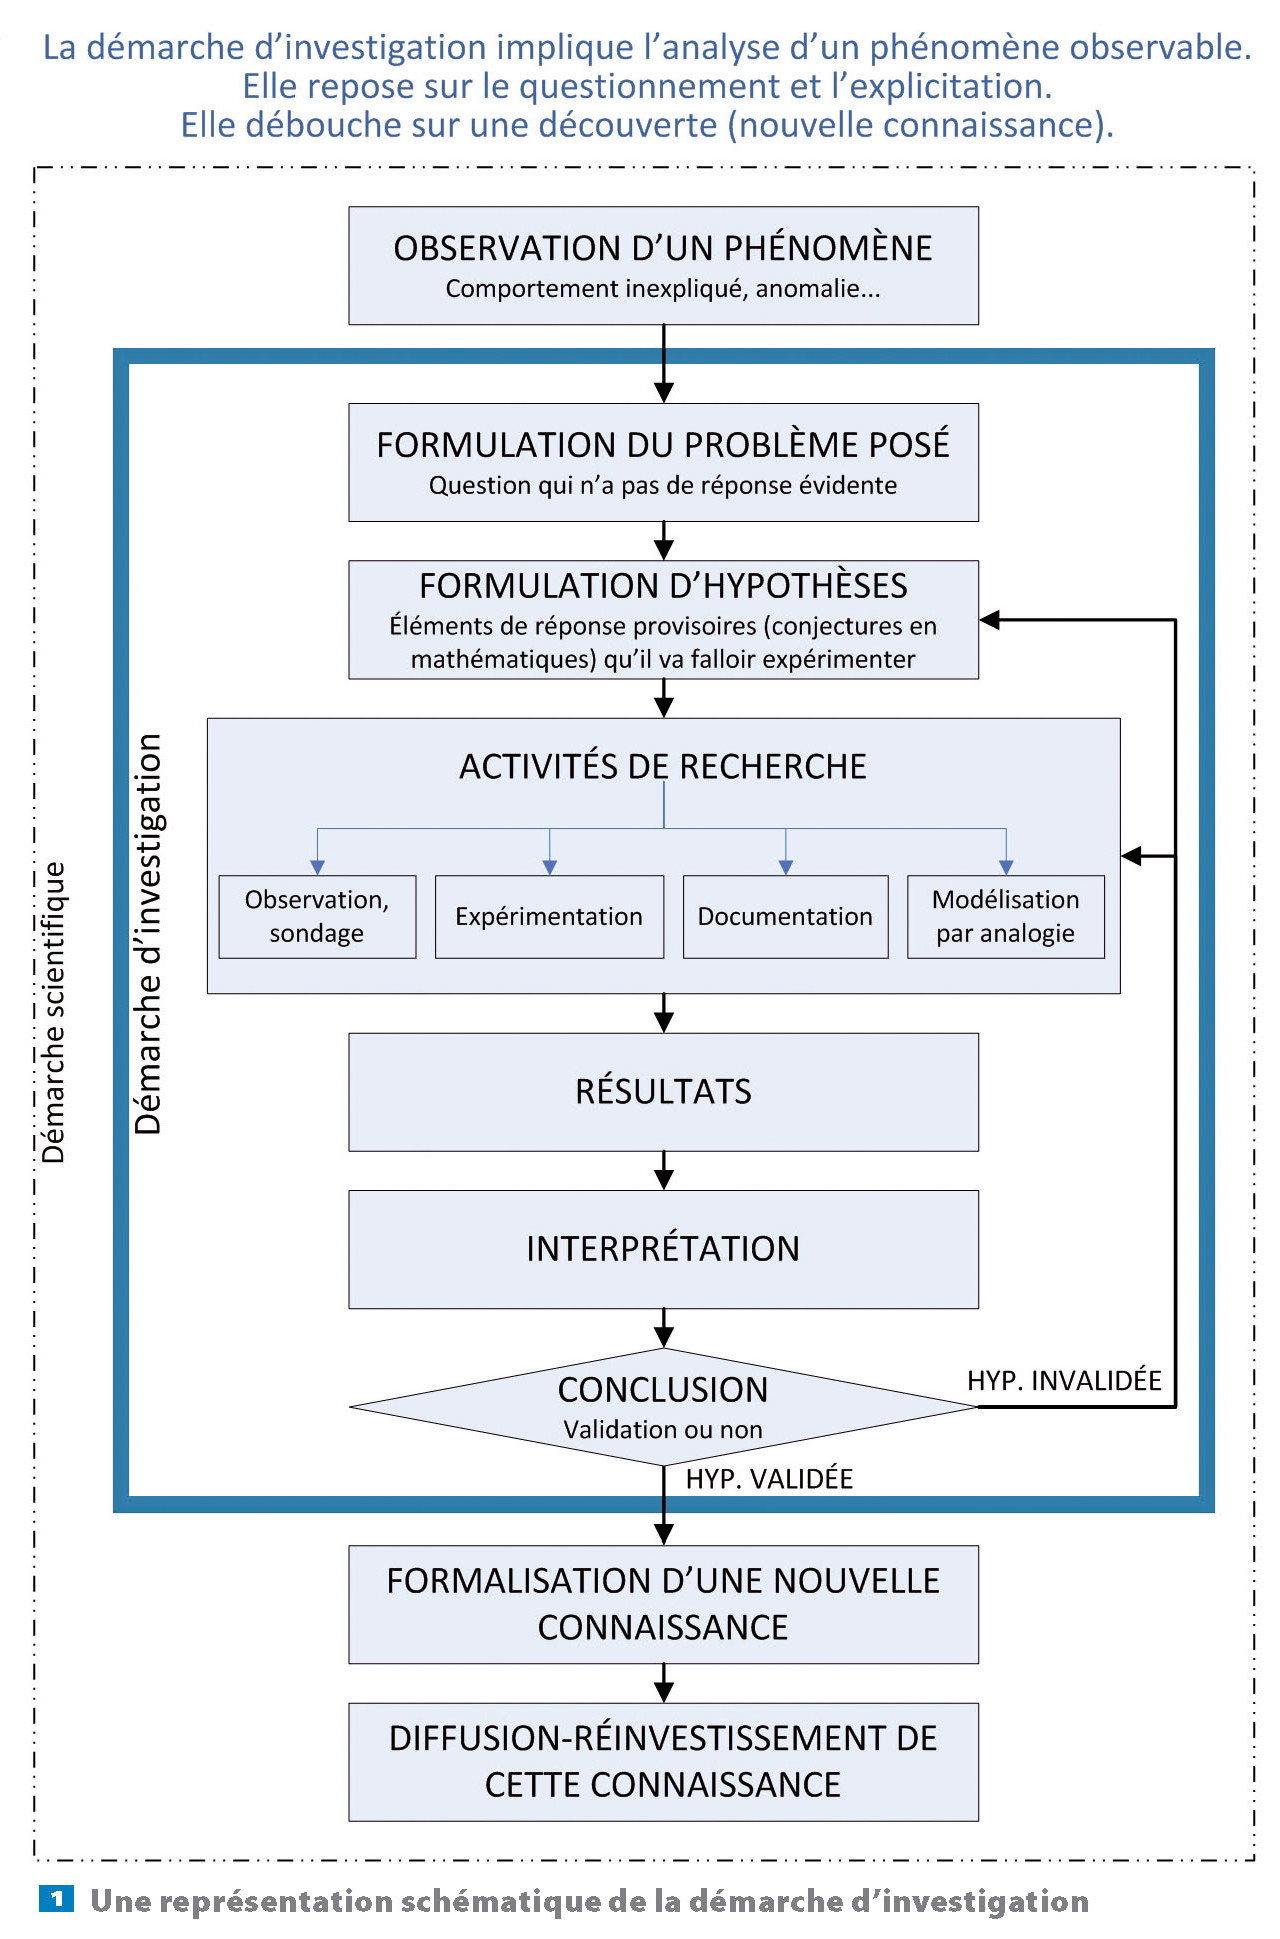
\includegraphics[width=\textwidth]{718-revue-technologie-n177-p59}
	
	\label{demarcheSci}
	\vfill
	\mbox{}
}{%
	\centering
	\noindent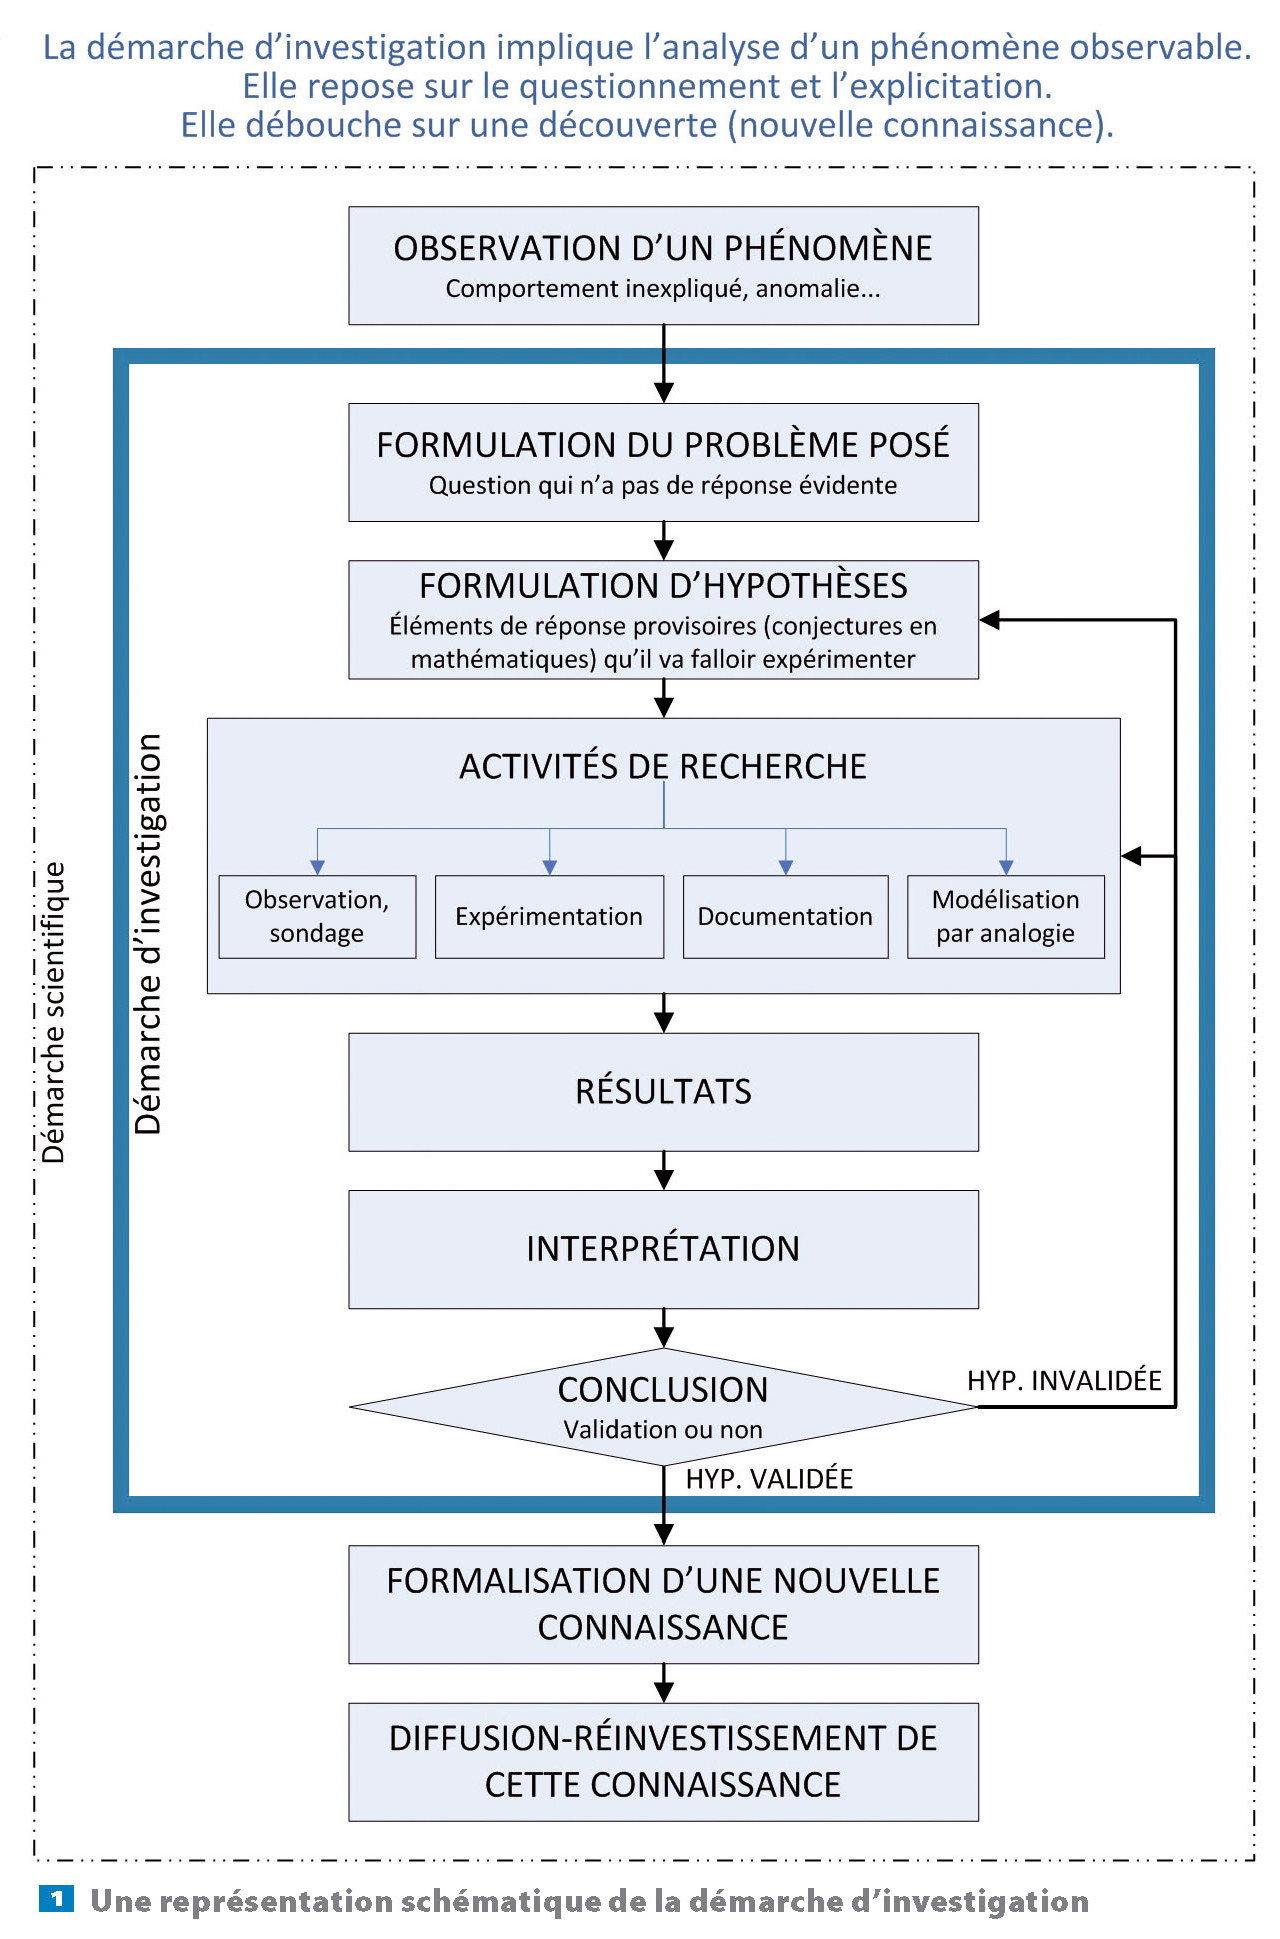
\includegraphics[height=\textheight]{718-revue-technologie-n177-p59}
	
	\label{demarcheSci}
}
	\ifthenelse{\boolean{papier}}{\clearemptydoublepage}{\newpage}
\ifthenelse{\boolean{caco}}{}{\thispagestyle{empty}}
\
\vfill 
\begin{center}
	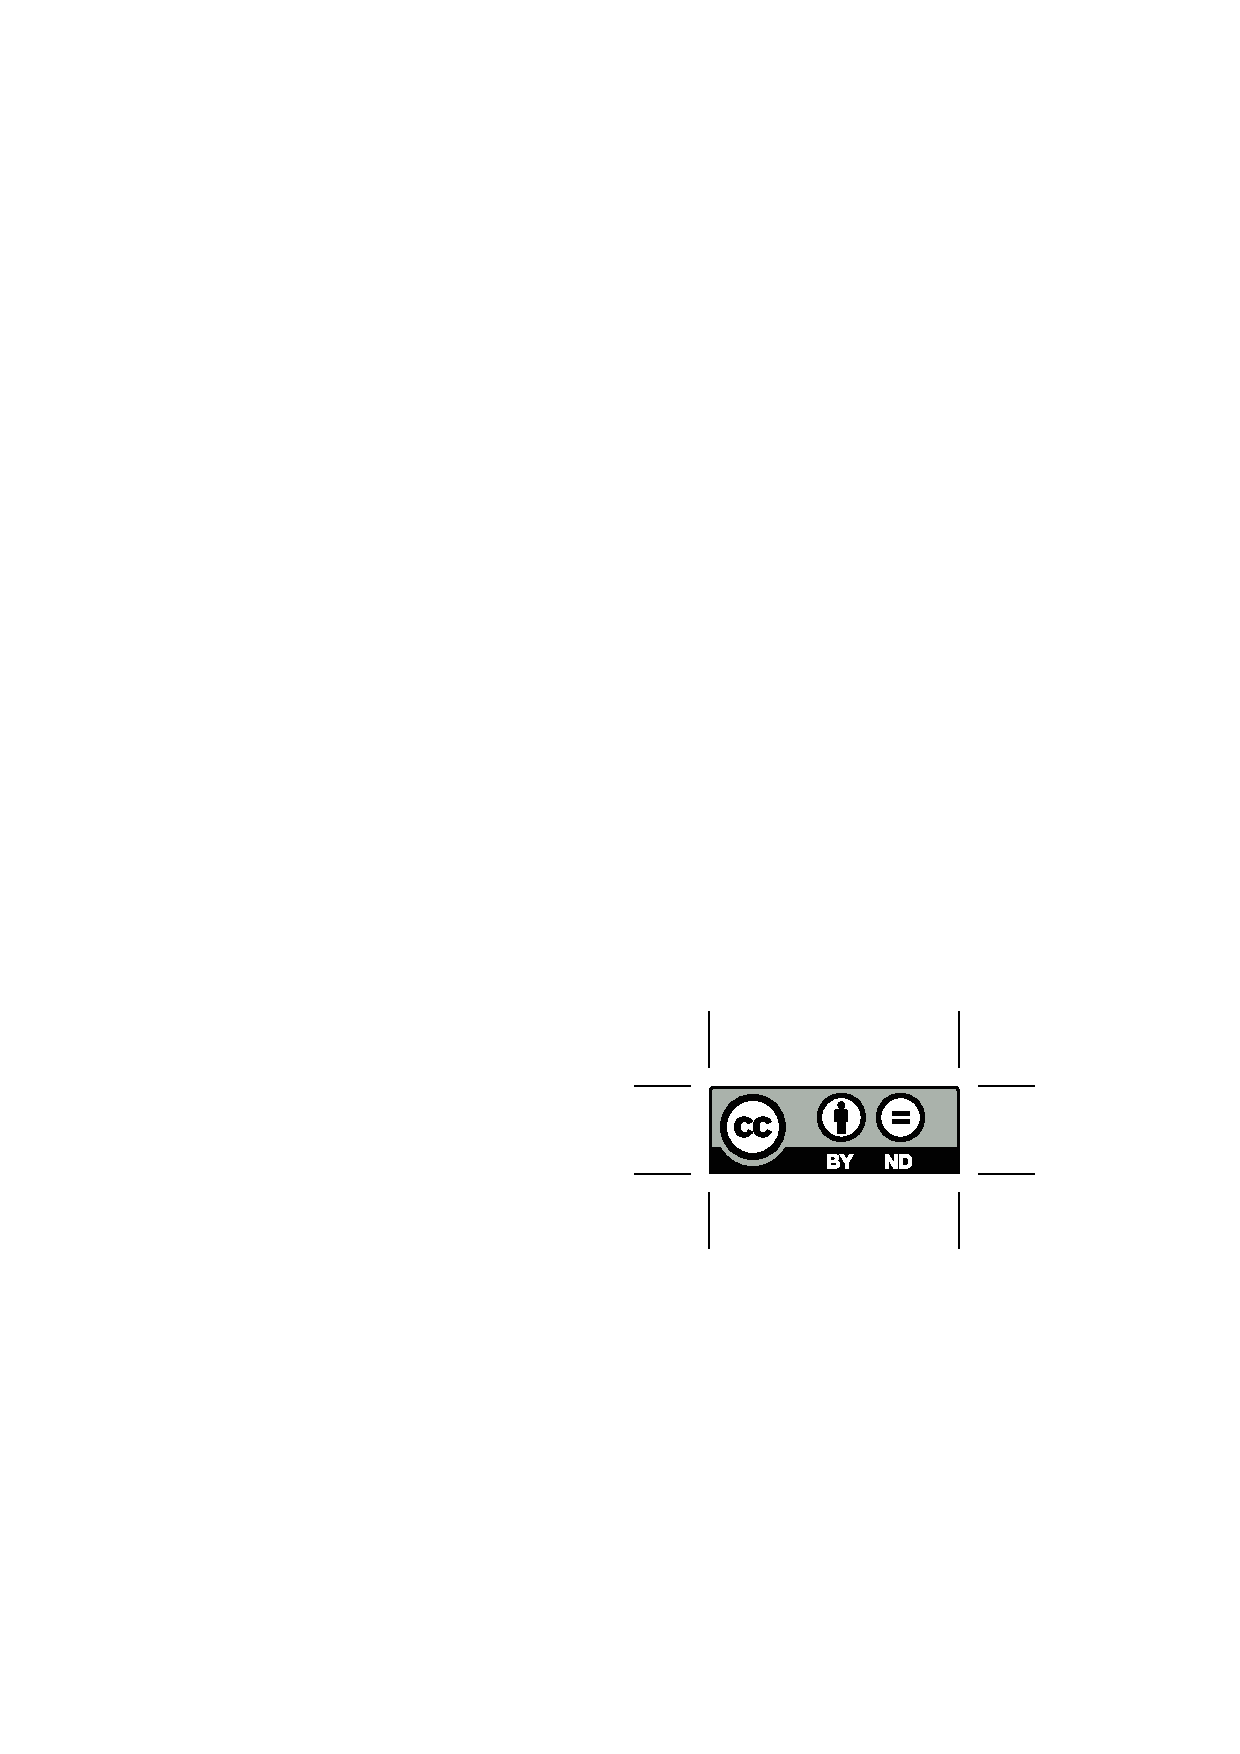
\includegraphics[height=35px]{by-nd}\\[1em]
	Cette œuvre est mise à disposition selon les termes de la licence Creative Commons Attribution -- Pas de Modification 4.0 International \url{http://creativecommons.org/licenses/by-nd/4.0/deed.fr}
\end{center}
	\def\grabtimezone #1#2#3#4#5#6#7#8#9{\grabtimezoneB}
\def\grabtimezoneB #1#2#3#4#5#6#7{\grabtimezoneC}
\def\grabtimezoneC #1#2'#3'{UTC#1#2\string:#3}
\thispagestyle{empty}
Ce document, composé en \LaTeX{} avec la police de caractères Latin Modern en corps~12, a été compilé le \today{} à \thistime[\ h\ ]
%    UTC+00\string:00.%sharelatex
\expandafter\grabtimezone\pdfcreationdate.
	%\ifthenelse{\boolean{papier}}{\clearemptydoublepage}{}
\ifthenelse{\boolean{caco}}{%
	\mbox{}\newpage
	\ifodd\thepage ~\newpage~\fi
	}{\chapter*{Résumé}}
Le programme d’enseignement de l’école primaire spécifie la démarche d’investigation pour l’enseignement des sciences au cycle~3, le site internet du Ministère de l’Éducation nationale, de l’Enseignement supérieur et de la Recherche préconise une initiation à la démarche d’investigation dès la maternelle, et le socle commun de connaissances et de compétences qui se retrouve dans le code de l’éducation fait référence à l’opération \og La main à la pâte \fg{} pour l’enseignement des sciences. D'après notre enquête, l’enseignement des sciences se fait effectivement dès la maternelle en utilisant cette démarche, et le nombre d’heures consacrées est proche du nombre d’heures consacré aux sciences au cycle~2. Néanmoins les dérives soulignées par le \textit{Rapport sur l’opération \og La main à la pâte \fg{} et l’enseignement des sciences à l’école primaire} sont toujours d’actualité. Il s’agit de la dérive du \og tout méthodologique \fg{} où l’utilisation de la démarche est privilégiée à l’acquisition des connaissances, ainsi que la dérive du \og tout technologique \fg{} où le seul but est de construire un objet sans que cela réponde à une problématique.

\begin{description}
\item[Mots-clés:] Éducation, sciences, maternelle, démarche d’investigation, La main à la pâte
\end{description}
\vfill
\ifthenelse{\boolean{papier}}{\clearemptydoublepage}{}
\ifthenelse{\boolean{caco}}{}{\chapter*{Abstract}}
\selectlanguage{english}
The curriculum of primary school specify the investigative approach for cycle~III (8–10 years of age), the website of the Ministry of National Education, Higher Education and Research recommends an introduction to the investigative approach in pre-school (3–5 years of age), and the Common Base of Knowledge and Skills that is found in the Education Code refers to the ``Hands on'' operation for teaching Science. According to our survey, science teaching in pre-school is actually using this approach, and the number of hours spent is close to the number of hours devoted to science in cycle II (6–7 years of age). Nevertheless drifts highlighted by the \textit{Report on the ``Hands on'' operation and science education in primary school} are still relevant. It is the drift of ``all methodological'' where the use of the approach is preferred to the acquisition of knowledge and the drift of ``all technological'' where the only goal is to construct an object that is not consistent with a problem.

\begin{description}
\item[Keywords:] Education, science, pre-school, investigation approach, Hands on
\end{description}
\selectlanguage{french}
\vfill
\end{document}

http://www.troubleshooting-tex.de
http://lesfichesabebert.fr/index.php/Koma/Koma-Script

http://educationdidactique.revues.org/510